\documentclass{vldb}
%\usepackage{graphicx}
\usepackage{balance}  % for  \balance command ON LAST PAGE  (only there!)

%\newtheorem{observation}{Observation}
%\newtheorem{claim}{Claim}
%\newtheorem{conjecture}{Conjecture}
%\newtheorem{problem}{Problem}
%\newtheorem{algo}{Algorithm}
%\newtheorem{definition}{Definition}
%\newtheorem{lemma}{Lemma}
%\newtheorem{theorem}{Theorem}
%\newtheorem{proof}{Proof}
%\newtheorem{defi}{Definition}

\newcommand\independent{\protect\mathpalette{\protect\independenT}{\perp}}
\def\independenT#1#2{\mathrel{\setbox0\hbox{$#1#2$}%
\copy0\kern-\wd0\mkern4mu\box0}} 

\newcommand{\atiter}[2]{{#1}^{(#2)}}
\newcommand{\itert}[1]{{#1}^{(t)}}
\newcommand{\itertO}[1]{{#1}^{(t+1)}}
\newcommand{\iiter}[1]{{#1}^{(i)}}
% \newcommand{\raiseTheta}[1]{\theta^{#1}}
\newcommand{\raisePsi}[1]{\psi^{#1}}
\newcommand{\order}[1]{\mathcal{O}(#1)}

\newcommand{\hide}[1]{}
\newcommand{\comment}[1]{\textcolor{red}{{\small #1 }}}
\newcommand{\semihide}[1]{{\tiny #1}}
\newcommand{\reminder}[1]{{\textsf{\textcolor{red}{[#1]}}}}
\newcommand{\makeclean}{
    \renewcommand{\reminder}[1]{}
}

%\newcommand{\QED}{ \hfill {\bf QED}}
\newcommand{\tight}{ \setlength{\itemsep}{-1.0\itemsep} }
    % makes lists tighter

\usepackage[mathscr]{eucal} %% For \mathscr
\usepackage{amsbsy} %% For \boldsymbol
\newcommand{\tensor}[1]{\boldsymbol{\mathscr{#1}}}   %% Tensor macro from Tammy
% \newcommand{\tensor}[1]{{\boldmath\mathcal{#1}}}
\newcommand{\B}[1]{\mathbf{#1}}   %% Tensor macro from Tammy
%\newcommand{\tensor}[1]{\underline{\mathbf{#1}}}  
%\newcommand{\tensor}[1]{\mathbf{\EuScript{#1}}}  
%\newcommand{\tensor}[1]{\mathbf{\mathcal{#1}}}  
\newcommand{\loss}{\mathcal{L}}  

\newcommand{\krp}[2]{ \left( \mathbf{#1}\odot\mathbf{#2} \right)}

\def\blambda{\mbox{\boldmath ${\lambda}$}}

\newcommand{\method}{\textsc{METHOD}\xspace}
\newcommand{\methodplain}{METHOD\xspace}
\newcommand{\graphlab}{GraphLab\xspace}
\newcommand{\psgd}{PSGD\xspace}
\newcommand{\dsgd}{DSGD+\xspace}
\newcommand{\lda}{LDA\xspace}
\newcommand{\dl}{DL\xspace}
\newcommand{\mmsb}{MMSB\xspace}
\newcommand{\twitter}{TGraph\xspace}
\newcommand{\nytimes}{NyTimes\xspace}
\newcommand{\snytimes}[1]{NyTimes{#1}\xspace}
\newcommand{\scaleblenytimes}{Scalable NyTimes\xspace}
\newcommand{\pubmed}{PubMed\xspace}
\newcommand{\imagenet}{ImageNet\xspace}

\newcommand{\sgd}{SGD\xspace}

%\newcommand{\explosion}{\textsc{Idex}\xspace}
\newcommand{\explosion}{intermediate data explosion\xspace}
\newcommand{\Explosion}{Intermediate Data Explosion\xspace}
\newcommand{\gtscaleup}{100\xspace}

\newcommand{\samplecube}{\textsc{ParCube}\xspace}
\newcommand{\parafac}{\textsc{Parafac}\xspace}
\newcommand{\sparafac}{\textsc{Parafac SLF}\xspace}
\newcommand{\merge}{\textsc{Merge}\xspace}
\newcommand{\sample}{\textsc{BiasedSample}\xspace}
\newcommand{\enron}{\textsc{Enron}\xspace}
\newcommand{\facebook}{\textsc{Facebook}\xspace}
\newcommand{\lbnl}{\textsc{Lbnl}\xspace}
\newcommand{\nell}{\textsc{Nell}\xspace}
\newcommand{\argmin}{\text{argmin}\xspace}
\newcommand{\brain}{\textsc{BrainQ}\xspace}


\newcommand{\hadi}{{\cal HADI}\xspace}
\newcommand{\mapreduce}{\textsc{MapReduce}\xspace}
\newcommand{\map}{\textsc{Map}\xspace}
\newcommand{\reduce}{\textsc{Reduce}\xspace}
\newcommand{\combine}{\textsc{Combine}\xspace}
\newcommand{\hadoop}{\textsc{Hadoop}\xspace}
\newcommand{\anf}{\emph{Centralized Method}}
% \newcommand{\MFB}{{MF-bitstring}}
\newcommand{\MFB}{{FM-bitstring}}
\newcommand{\mfb}{{b}}
\newcommand{\MFV}{{FM-vector}}
\newcommand{\mfv}{{\bf v}}
% \newcommand{\mfbhi}{{MF-vector}}
\newcommand{\mfbhi}{{ b(h,i) }}
\newcommand{\Nhi}{N(h,i)}   % number of neighbors of $i$, within h hops or less
\newcommand{\NNhi}{ {\cal N}(h,i)} % SET of neighbors ....
\newcommand{\NNhhi}{ {\cal N}(h+1,i)} % SET of neighbors ....
\newcommand{\NNhj}{ {\cal N}(h,j)} % SET of neighbors ....
\newcommand{\hatmfbhi}{ $\hat{b}(h,i)$} %partial bitmask

\newcommand{\PassA}{{\tt Stage1}\xspace}
\newcommand{\PassAMap}{{\tt Stage1-Map}\xspace}
\newcommand{\PassARed}{{\tt Stage1-Reduce}\xspace}
\newcommand{\PassB}{{\tt Stage2}\xspace}
\newcommand{\PassBMap}{{\tt Stage2-Map}\xspace}
\newcommand{\PassBRed}{{\tt Stage2-Reduce}\xspace}
\newcommand{\PassC}{{\tt Stage3}\xspace}
\newcommand{\PassCMap}{{\tt Stage3-Map}\xspace}
\newcommand{\PassCRed}{{\tt Stage3-Reduce}\xspace}

\newcommand{\diameter}{{\tt diameter}}
\newcommand{\npairs}{{\tt npairs}}
\newcommand{\gcc}{{\tt gcc}}
\newcommand{\entropy}{{\tt entropy}}
% \newcommand{\nedges}{{\tt nedges}}
\newcommand{\sv}{{\mbox{$\lambda_1$}}}
\newcommand{\avgd}{{\tt avgd}}

% math symbol definitions
\newcommand{\mat}[1]{{\bf{#1}}}
\newcommand{\nnodes}{N}     % number of nodes
\newcommand{\nedges}{E}     % number of edges
\newcommand{\deff}{{d_{eff}}}   % effective diameter
\newcommand{\Er}{{E_{r}}}   % number of retained edges
\newcommand{\Nr}{{N_{r}}}   % number of retained nodes
\newcommand{\Nc}{{N_c}}   % number of nodes at critical point
\newcommand{\Ec}{{E_c}}   % number of nodes at critical point
\newcommand{\Ngcc}{{N_{gcc}}} % number of nodes in gcc, at critical poing
\newcommand{\NPairc}{{N_{NPAIRS}}} % number of reachable pairs, at critical poing
\newcommand{\dc}{{d_{c}}} % diameter at critical point
\newcommand{\Lambdac}{{\lambda_{c}}} % First eigenvalue at critical point
% \newcommand{\RED}{ {\em RED } } % random edge deletion
% \newcommand{\FED}{ {\em FED } } % friendly edge deletion
% \newcommand{\HED}{ {\em HED } } % hostile edge deletion
\newcommand{\join}{\texttt{combine2}}
\newcommand{\aggrnp}{\texttt{combineAll}}
\newcommand{\aggr}{\texttt{combineAll$_i$}}
\newcommand{\aggrsid}{\texttt{combineAll$_{E.sid}$}}
\newcommand{\assign}{\texttt{assign}}



\newcommand{\ben}{\begin{enumerate*}}
\newcommand{\een}{\end{enumerate*}}
\newcommand{\bit}{\begin{itemize*}}
\newcommand{\eit}{\end{itemize*}}

% shorthands
\newcommand{\citationsds}{{CITATIONS}}
\newcommand{\epinionsds}{{EPINIONS}}
\newcommand{\patentsds}{{PATENTS}}
\newcommand{\net}[1]{{\textsc{#1}}}

\newcommand{\QED}{\hfill $\Box$ \hfill}





% graph segment
% Notation macros
\newcommand{\G}{\ensuremath{{\mathcal G}}}  % graph stream
\newcommand{\ES}[1]{\ensuremath{m^{(\!#1\!)}}}
%\newcommand{\ES}[1]{\ensuremath{|E|^{(\!#1\!)}}}
\newcommand{\coll}{\ensuremath{\ell}}  % number of source/row groups
\newcommand{\rowk}{\ensuremath{k}}  % number of dest/col groups
\newcommand{\rgrp}[1]{\ensuremath{I^{(\!#1\!)}}}  % node set for src/row group
\newcommand{\cgrp}[1]{\ensuremath{J^{(\!#1\!)}}} % node set for dst/col group
\newcommand{\rgsz}[1]{\ensuremath{l^{(\!#1\!)}}}  % size of node set for src/row group
\newcommand{\cgsz}[1]{\ensuremath{n^{(\!#1\!)}}  }% size of node set for dst/col group
\newcommand{\subG}[1]{\ensuremath{{\mathcal G}^{(\!#1\!)}}}  % submatrices
\newcommand{\den}[1]{\ensuremath{\rho^{(\!#1\!)}}}   % density/probability
\newcommand{\KL}[2]{\ensuremath{{\mathcal D}(#1\|#2)}}   % KL-divergence
\newcommand{\ceil}[1]{\ensuremath{\lceil\!#1\!\rceil}}   % density/probability

\newcommand{\myrot}[1]{\rotatebox[origin=ll]{75}{{#1}}} 


\usepackage{amsmath,amsfonts,amssymb}
\usepackage{subfigure,grffile,placeins}
\usepackage{graphicx} 
\usepackage{epstopdf}
\usepackage{hyperref}
\usepackage{wrapfig}
\usepackage[lined,boxed]{algorithm2e}
\usepackage{url}
\usepackage{xcolor}
\usepackage{tikz}
\usepackage{xkeyval} 
%\usepackage{pax}
%\usepackage{pdfpages}
%\usetikzlibrary{shadows}
%\usetikzlibrary{shapes,arrows,decorations.pathmorphing,backgrounds,fit,positioning}
%\tikzstyle{every picture}+=[remember picture]


\newtheorem{observation}{Observation}
\newtheorem{conjecture}{Conjecture}
\newtheorem{problem}{Problem Definition}
\newtheorem{algo}{Algorithm}
\newtheorem{definition}{Definition}
\newtheorem{lemma}{Lemma}
\newtheorem{theorem}{Theorem}
\newtheorem{assumption}{Assumption}
%\newtheorem{question}{Question}
\newtheorem{example}{Example}
\newcommand{\pushright}[1]{\ifmeasuring@#1\else\omit\hfill$\displaystyle#1$\fi\ignorespaces}
\newcommand{\pushleft}[1]{\ifmeasuring@#1\else\omit$\displaystyle#1$\hfill\fi\ignorespaces}

%\newtheorem{answer}{Answer}
%\newtheorem{proof}{Proof}

\newcommand{\abhi}[1]{\textcolor{orange}{abhi-comment: #1}}
\newcommand{\alex}[1]{\textcolor{red}{alex-comment: #1}}
\newcommand{\qirong}[1][1]{\textcolor{fuschia}{\\ qirong-comment: #1}}
\newcommand{\eric}[1][1]{\textcolor{blue}{\\ eric-comment: #1}}


\pgfdeclareimage[height=0.5in]{machine}{figs/server2.png}


\begin{document}

% ****************** TITLE ****************************************

\title{\methodplain: A General Optimization Framework for Fast, Scalable Machine Learning}

% possible, but not really needed or used for PVLDB:
%\subtitle{[Extended Abstract]
%\titlenote{A full version of this paper is available as\textit{Author's Guide to Preparing ACM SIG Proceedings Using \LaTeX$2_\epsilon$\ and BibTeX} at \texttt{www.acm.org/eaddress.htm}}}

% ****************** AUTHORS **************************************

% You need the command \numberofauthors to handle the 'placement
% and alignment' of the authors beneath the title.
%
% For aesthetic reasons, we recommend 'three authors at a time'
% i.e. three 'name/affiliation blocks' be placed beneath the title.
%
% NOTE: You are NOT restricted in how many 'rows' of
% "name/affiliations" may appear. We just ask that you restrict
% the number of 'columns' to three.
%
% Because of the available 'opening page real-estate'
% we ask you to refrain from putting more than six authors
% (two rows with three columns) beneath the article title.
% More than six makes the first-page appear very cluttered indeed.
%
% Use the \alignauthor commands to handle the names
% and affiliations for an 'aesthetic maximum' of six authors.
% Add names, affiliations, addresses for
% the seventh etc. author(s) as the argument for the
% \additionalauthors command.
% These 'additional authors' will be output/set for you
% without further effort on your part as the last section in
% the body of your article BEFORE References or any Appendices.

\numberofauthors{3} %  in this sample file, there are a *total*
% of EIGHT authors. SIX appear on the 'first-page' (for formatting
% reasons) and the remaining two appear in the \additionalauthors section.

\author{
% You can go ahead and credit any number of authors here,
% e.g. one 'row of three' or two rows (consisting of one row of three
% and a second row of one, two or three).
%
% The command \alignauthor (no curly braces needed) should
% precede each author name, affiliation/snail-mail address and
% e-mail address. Additionally, tag each line of
% affiliation/address with \affaddr, and tag the
% e-mail address with \email.
%
% 1st. author
\alignauthor
Abhimanu Kumar\titlenote{\label{note1}The first two authors contributed equally to this work.}\\
       \affaddr{School of Computer Science}\\
       \affaddr{Carnegie Mellon University}\\
       \affaddr{Pittsburgh, PA}\\
       \email{abhimank@cs.cmu.edu}
% 2nd. author
\alignauthor
Alex Beutel\raisebox{9pt}{$\ast$} \\
       \affaddr{School of Computer Science}\\
       \affaddr{Carnegie Mellon University}\\
       \affaddr{Pittsburgh, PA}\\
       \email{abeutel@cs.cmu.edu}
% 3rd. author
\alignauthor 
Qirong Ho\\
       \affaddr{School of Computer Science}\\
       \affaddr{Carnegie Mellon University}\\
       \affaddr{Pittsburgh, PA}\\
       \email{qho@cs.cmu.edu}
\and  % use '\and' if you need 'another row' of author names
% 4th. author
\alignauthor 
Eric P. Xing\\
       \affaddr{School of Computer Science}\\
       \affaddr{Carnegie Mellon University}\\
       \affaddr{Pittsburgh, PA}\\
       \email{epxing@cs.cmu.edu}
}
% There's nothing stopping you putting the seventh, eighth, etc.
% author on the opening page (as the 'third row') but we ask,
% for aesthetic reasons that you place these 'additional authors'
% in the \additional authors block, viz.
%\additionalauthors{Additional authors: John Smith (The Th{\o}rv\"{a}ld Group, {\texttt{jsmith@affiliation.org}}), Julius P.~Kumquat
%(The \raggedright{Kumquat} Consortium, {\small \texttt{jpkumquat@consortium.net}}), and Ahmet Sacan (Drexel University, {\small \texttt{ahmetdevel@gmail.com}})}
%\date{30 July 1999}
% Just remember to make sure that the TOTAL number of authors
% is the number that will appear on the first page PLUS the
% number that will appear in the \additionalauthors section.


\maketitle

\begin{abstract}
	How can Facebook scalably model their billion-node social network?  How
can Twitter efficiently run a topic model over billions of tweets?
``Big data'' today does not just mean more data to mine but also more things
to understand - more users, more documents, more images.
Modern machine learning and data mining faces the challenge of
scaling our classic models to both use all of the data available as well as build
larger and more complex models of our world. 
%In modern machine learning and data mining using models,
%which were designed for thousands of items, on billions of items is a constant
%challenge.  
%The big data revolution pushes our systems to not only be able to
%process moredata but also to be able to fit larger and more complex models.  
%Our ``documents'' in topic modeling tweets are shorter not longer and our
%social circles are not growing exponentially, but we have so many more of them
%requiring our models to scale with the data being produced.

In this paper we describe \method, a general framework for performing fast
machine learning on huge models and big data.  Our system uses a combination
of recent insights in stochastic learning theory to enable our
system innovations.  In particular, our system offers three contributions:
{\bf (1) Scalability:} Our system distributes both the data and model across
the cluster of machines, allowing the system to scale to terrabytes of data as
well as models with billions of parameters. {\bf (2) Versatility:} Our system supports
synchronized parameter updates, such as normalizing across the cluster.
As a result, we can fit a variety of machine learning models, including topic
models, dictionary learning, and mixed membership stochastic block models.
{\bf (3) Speed:} We use a \textcolor{red}{modification} of stochastic gradient
descent, called Always-On SGD, to continously improve our model fit, even if
there are slow workers that would otherwise obstruct model synchronization and
slow computation. 
Finally, we demonstrate that with our new approah, \method can fit ML models at
an unprecedented scale and faster than prior work.

\end{abstract}

\section{Introduction} % (fold)
\label{sec:intro}
%\alex{\textbf{NOTE: The paper outline is still {\it very} rough, and I expect to re-order
%many sections, largely in attempt to keep the focus on the system.}}

\begin{figure}
	\centering
	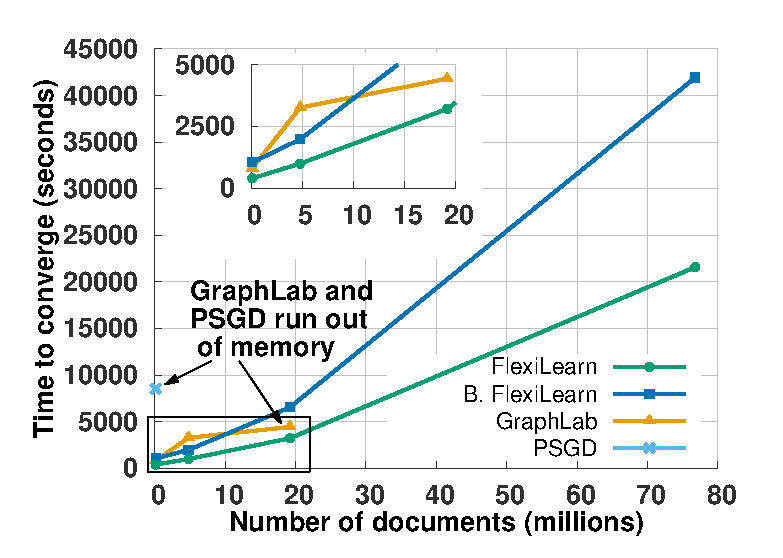
\includegraphics[width=0.8\columnwidth]{fig2/lda_datasize.eps}
	\caption{Scalability comparison for topic modeling}
	\label{fig:crownjewel}
\end{figure}

In recent years, the amount of data being produced and stored throughout the
world has exploded.  From science to e-commerce to news to social networking,
we, as a culture, are spending more time and money producing uniquely digital
content and recording elements of our physical world online for posterity and
analysis.  With this big data boom, the focus is often on the size of the data
- ``LHC produced 13 petabytes \ldots of data in
2010\footnote{\url{http://www.nature.com/news/2011/110119/full/469282a.html}}''
and ``500+terabytes of new data ingested into [Facebook] databases every
day\footnote{\url{http://gigaom.com/2012/08/22/facebook-is-collecting-your-data-500-terabytes-a-day/}}.''
While handling all of this data is an important challenge and lots of work has
focused on scaling to large datasets, this misses an important part of the
picture - we are also recording more data about {\em more things}: ``300
million photos uploaded per day [to Facebook]'' and there are more than 400
million tweets sent per
day\footnote{\url{http://articles.washingtonpost.com/2013-03-21/business/37889387_1_tweets-jack-dorsey-twitter}}.
The challenge now becomes not just using all of the data, but also
understanding all of these items.

Machine learning has focused on understanding large datasets for many years
now, but the research often ignore the challenge of scaling to models over many
millions or even billions of items, e.g. finding the topics of millions of news
articles, removing noise from the many images upoaded online, or clustering users
in a billion node social network.  In each of these cases, the issue is not
just the size of the data but also the number of items we need to model and
understand.  Even if we distribute our dataset across many machines, the model
of topics for 100 million documents (news articles or webpages) across even 100
topics would take over 35 gigabytes just to store in memory.  

In this paper we describe a new system, \method, for answering such complex
questions about modern massive datasets.  Informally and generally,
the problem we are solving is:\\ 
\textbf{Given:} A database of relations between different objects\\
\textbf{Find:} A model of those objects which best matches those relationionships.\\
As an example, for the special case of topic modelling this can be framed, again informally, as:\\
\textbf{Given:} A database of documents for which we know the use of different words in different documents\\
\textbf{Find:} The probability of each document being about a particular topic,
and for each topic the probability that a word is used when discussing that topic.\\
We define our problem formally as a minimization problem over a class of functions in
Section \ref{sec:mdAbstract}.  

In order to answer a variety of such complex questions, \method focuses on a
new abstraction for relational data that enables easy partitioning and
distribution of both the dataset and model across a cluster of machines.  This
abstraction for relational data is flexible enough to answer a wide variety of
common machine learning queries.  In this paper we describe the following
contributions:
\begin{enumerate}
	\item \textbf{Scalability:} Our system scales to model billions of items
		using massive datasets.  We are particularly efficient in our memory
		usage, enabling us to scale beyond current state of the art systems.
	\item \textbf{Versatility:} \method can answer a wide variety of complex
		machine learning queries, often with even higher accuracy than other
		systems.  We demonstrate our effectiveness on topic modeling,
		dictionary learning for de-noising images, and mixed membership
		stochastic block models for clustering users in a network.
	\item \textbf{Speed:} We use new techniques for running over barriers to
		not waste computational time even when waiting stragglers in the cluster.
		This lets \method converge to the final answer faster than
		competitors.
	\item \textbf{Portability:} Because of Apache's Hadoop
		and HDFS ubiquity in industry, we build our system on top of these
		frameworks.  This makes it extremely easy to run the system without
		having to modify your cluster.
\end{enumerate}

In Section \ref{sec:mdAbstract} we explain our scalable abstraction for the
model and data, and give the high level overview of computation under this
abstraction in a cluster.  In Section \ref{sec:learning} we give the background
on different learning techniques, such as gradient based learning, for modeling
our data.  In Section \ref{sec:complexQues} we describe how our system can
answer a wide variety of complex questions, such as what is the probability of
a webpage being about a set of topics.  In Section \ref{sec:overBarriers} we
explain how we can continue performing valuable computation even while waiting
for stragglers to catch up, thus enabling our system to converge to the solution
quickly.  In Section \ref{sec:implementation} we give the details of how we
implemented the system on Hadoop.  In Section \ref{sec:applications} we
describe a few different applications of our system and in Section
\ref{sec:experiments} we describe our experimental setup.  In Section
\ref{sec:eval} we evaluate our system against other state of the art systems.
Finally in Section \ref{sec:related} we give a survey of the related work, and we
conclude in Section \ref{sec:conclusion}.


\section{Problem definition} % (fold)
\label{sec:problem}
For many classic machine learning problems, we have data about the
relationships between different types of objects and we would like to
understand these objects and their relationship to each other.  We consider we
have $t$ sets of objects $\mathcal{T}_1, \mathcal{T}_2, \ldots \mathcal{T}_t$,
each with $T_i = |\mathcal{T}_i|$ items which can be indexed from $j=1$ to $T_i$ as $\mathcal{T}_{i,j}$.
From this we have a dataset of relations between these objects defined by
$$\mathcal{X}: \mathcal{T}_1 \times \mathcal{T}_2\times \ldots \times \mathcal{T}_n \rightarrow \mathbb{R}.$$

Given such a dataset, we would like to find a set of values for each object
to describe that object.  Therefore, we have also $t$ sets of variables
$\Theta = \{\theta_1 \ldots \theta_t\}$ where $\theta_{i,j}$ is a set of
variables (often a vector) which describe object $\mathcal{T}_{i,j}$.  For
notational simplicity, we will say that given a vector of indices
$\mathbf{i}=(i_1,i_2,\ldots i_t)$ we can reference the relevant variables by
$\Theta_{\mathbf{i}} = \{\theta_{1,\mathbf{i}_1},\theta_{2,\mathbf{i}_2}, \ldots \theta_{t,\mathbf{i}_t} \}$.

We can now formally define our general problem:
\vspace{-2mm}
\begin{problem}
	Given dataset $\mathcal{X}$ defined over $t$ types of objects
	$\mathcal{T}$, our objective is to find $\Theta$ through the following
	minimization:
	\begin{align}
		%\arg\min_{\Theta} &\sum_{\mathbf{i} \in \{\mathcal{T}_1 \times \mathcal{T}_2 \times \ldots \times \mathcal{T}_t\}} f(\Theta_\mathbf{i},\mathcal{X}(\mathbf{i}))\\
		\arg\min_{\Theta} &\sum_{\mathbf{i} \in \mathcal{X}} f(\Theta_\mathbf{i},\mathcal{X}(\mathbf{i}))\\
		& {\rm s.t.}\; C(\Theta) = \mathbf{1},
	\end{align}
	where $f$ is any differentiable function and $C$ is a convex constraint
	across subsets of variables in $\Theta$.
\end{problem}
\vspace{-2mm}
Without loss of generality we can also set $\mathcal{T}_i = \mathcal{T}_j$ such
that we have relations between objects of the same type.  
Additionally, we can combine the loss function across multiple datasets on
similar objects by merely adding their objectives together. 

This problem defintion is very broad covering a variety of common problems as
special cases including topic modeling, dictionary learning, network
decomponsition, matrix and tensor factorization, and even mean field problems.
Throughout this paper, we will describe our system in terms of topic modeling
for clarity.  

\paragraph*{Special Case: Topic Modeling}
When performing topic modeling we have two types of objects ($t=2$) - words
and documents, which we will denote by $\mathcal{T}_1 = \mathcal{W}$ and
$\mathcal{T}_2=\mathcal{D}$.  
For each document $d\in\mathcal{D}$, we know the number of times a
word $w\in\mathcal{W}$ was used; our dataset $\mathcal{X}$ is the normalized version of these values.  
Our objective is to predict which words will be
used in which documents.  In the process, we attempt to find the topics of each
document and the words used when discussing each topic (from $K$ topics). 
To do this, we use the following model:
\begin{align*}
	p({\rm Word}\; w | {\rm Doc}\; d) = \sum_{ {\rm Topic}\; k = 1}^K p(w | {\rm Topic} \!=\! k)\cdot  p( {\rm Topic} \!=\! k | d)
\end{align*}
The variables for the probabilities that a word is used in discussing a given
topic are denoted by $\theta_1=\beta$, where $\beta_j$ is the $K$-length vector of
probabilities $p(w_j|{\rm Topic}= k)$ for all $k$.  Similarly the variables for
the probabilities that a document is about a given topic are denoted by
$\theta_2=\pi$ where $\pi_i$ is the $K$-length vector of probabilities
$p(d_i|{\rm Topic}=k)$ for all $k$.

From this, we have a similar problem statement as before but specific to topic modeling:
\begin{problem}
	Given a word $\times$ document dataset $\mathcal{X}$, find
	\begin{align}
		\arg\min_{\pi,\beta} &\sum_{d_i \in \mathcal{D},w_j \in \mathcal{W}} f(\pi_i,\beta_j,\mathcal{X}(i,j)) \label{eqn:LDA}\\
		f(\pi_i,\beta_j,x) &= (x - \pi_i\beta_j^\top)^2\\
		{\rm s.t.}\; &\sum_{k=1}^K \pi_{i,k} = 1,\; \forall d_i\in \mathcal{D}\\
		&\sum_{w_j \in \mathcal{W} } \beta_{j,k} = 1,\; \forall k = 1 \ldots K
	\end{align}
\end{problem}
Solving this produces a model of the topics of our documents and the use of our
words.  In particular, we are left with a model of the use of words in topics
given by $\beta$, which can be used to find the topics of new documents. 

In this topic model, the variables $\beta$ are an exclusive construct of the
model and are typically referred to as the model parameters.  These parameters
define our model of documents and can be used to model new documents once we
have learned our parameters.
In the general formulation of the problem earlier, for which we have a variety
object types $\mathcal{T}$, some subset of the variables in $\Theta$ are
typically considered to be model parameters.
%In the abstract 
%formulation of the problem earlier we introduced types $\mathcal{T}$. It is important to note 
%that some of these types are an exclusive construct of the model e.g. the topic-word 
%type $\beta$ in topic modelling. These types are called parameters of the model.
%\alex{ABHI: is this definition of parameters ok?}


% section Problem definition (end)

\section{Model and Data Abstraction}
\label{sec:mdAbstract}
In designing any large scale machine learning system, one of the most important
design decisions is the abstraction for the data and problem model.  Recent
distributed ML systems focus primarily on the abstraction for the data, such as
\graphlab's \cite{graphlab} view of each data point as a node or or
\psgd's view of partitioning only on the data.
Here we take a different approach - partitioning our data and the model we are building of the
data simultaneously.  As we will go on to demonstrate, focusing on both is
advantageous for both scalability and speed.

\subsection{Block structure in relational data} % (fold)
\label{sub:Block structure in relational data}

For many classic machine learning problems, we have relational data between
two sets of entities, and we are asking questions about these entities.  To be a
bit more concrete, consider the classic topic modeling question: given a large set
of $D$ documents, with what probability a given document talks about a given
topic, and with what probability does a given topic has a given word?  In this
case, a raw data point is the number of times a given word was used in a given document.
Each data point is an element in the document by word data matrix. We normalize
the data matrix to obtain matrix $Y$ where an element $Y_{i,j}$ in column $i$
and row $j$ in the new matrix is the original element at $(i,j)$ divided by 
the row $i$'s sum. In simple terms, $Y{i,j}$ is the probability of word $j$ 
lying in document $i$. 

We factorize $Y$ into two matrices $\pi$ and $\beta$. The $\pi$ matrix is the
per document topic probability matrix. $\pi_{i,k}$  is the probability that a given
document $i$ talks about topic $k$, or has topic $k$. The $\beta$ matrix is the
per topic word probability. $\beta_{k,j}$ is the probability of word $j$ present
in topic $k$. We are solving the following query to find $\pi$ and $\beta$.
{\small
\begin{align}
&\argmin_{\pi,\beta}L(Y,\pi,\beta)
=\sum_{i,j}(Y_{i,j}-\sum_k\pi_{i,k}\beta_{k,j})^2
%= \sum_{i,j}(Y_{i,j}-\sum_k \pi_{i,k}\beta_{k,j})_p^p
\label{eqn:LDA}\\
&\text{s.t.} \; \forall  i,j,k \quad
\sum_k\pi_{i,k}=1,
\sum_j\beta_{k,j}=1, \quad
\pi_{i,k}\geq 0,
\beta_{k,j}\geq 0,
\nonumber
\end{align}}

The equation~\ref{eqn:LDA} means that we want to approximate matrix $Y$ by the
product of matrices $\pi$ and $\beta$. The second line in
the equation is due to the fact that $\pi$ and $\beta$ are
probability matrices. 

Because of the intrinsic relational nature of the data (here between words and documents), partitioning our data ($Y$) intelligently results
in a clean partitioning of our model of topics for the words and documents.

More specifically, for any given subset of the documents and subset of the
words, there is a unique set of data points that are applicable to entities from
both sets.  If we view our data as a very sparse matrix $Y$ (where $Y$ is a
documents by word matrix), partitioning the documents and the words results in
the data matrix $Y$ also being partitioned into blocks, as seen in Figure
\ref{fig:abstraction}.
Under this partitioning, all data points in block $\mathcal{B}_{i,j}$ describe
a relationship between a word from set $\mathcal{S}^{(1)}_i$ and document from
set $\mathcal{S}^{(2)}_j$.  We focus our computation around these blocks of data.

An interesting property of these blocks is that for some blocks, such as
$\mathcal{B}_{i,j}$ and $\mathcal{B}_{i',j'}$ where $i\neq i'$ and $j \neq j'$,
we see that the blocks are \textit{independent}.  That is, a data point from
$\mathcal{B}_{i,j}$ does not describe any relations to words in
$\mathcal{S}^{(1)}_{i'}$ or documents in $\mathcal{S}^{(2)}_{j'}$ and vice
versa for data in $\mathcal{B}_{i',j'}$.
%Formally defined:
%\alex{add formal definition of independence here? or will that come off too
%mathy}
As has been shown in previous stochastic learning literature \cite{textbook}
and used in simpler data mining problems \cite{gemulla,flexifact}, this
independence property allows for improved scalability and parallel processing.
We will discuss our system and the strengths of this abstraction primarily in terms of topic modeling, 
%Note, we will primarily discuss
%this system in terms of topic modeling, 
but note the system generalizes to many
machine learning problems as we will demonstrate later.
%We go over the implications for topic modeling and other machine learning
%problems below.

\subsection{Distributing our data} % (fold)
\label{sub:Distributing the Data and Model}

As mentioned above, distributing your data over a cluster is useful, but as
data grows partitioning both the data and your model of that data is
increasingly valuable.  For example, if we would like to know the topic
distribution for 10 million documents over 1000 topics, this would require over
37 gigabytes just to hold all of the answers to the query.  Therefore, it is
crucial that as our data grows we intelligently distribute both the data and our
solution.  This significantly improve memory efficiency and makes it possible
to scale to unprecedented sizes.  Luckily, our blocking abstraction makes this
easy.

In processing a given block $\mathcal{B}_{i,j}$, we only need the data from
that block, and the current information about the words $\mathcal{S}^{(1)}_{i}$
and documents $\mathcal{S}^{(2)}_{j}$.  Therefore, in distributing the problem
over a cluster of machines, we can have each worker only store and process one
block and its corresponding object model at a time.  Additionally, because our
sets of documents and sets of words are each disjoint, we can process our
blocks in such a way that each document and each word is only being worked on
by one worker at a time.  As a result, we do not need to store \textit{any}
duplicate data (about the topic model or blocks) and thus we are perfectly
memory efficient.


% subsection Distributing the Data and Model (end)

\subsection{Parallel processing} % (fold)
The last piece of the general system design is understanding the order in which
we process our data.  Our goal is to reach the optimal memory efficiency
described above and also keep our computation fast and accurate.  To do this,
we must choose a \textit{stratum}, a group of blocks, to process in parallel.  
In order to be memory efficient and keep our computation accurate, each stratum
must only contain blocks that are independent of each other.  From the block
structure, we can create multiple strata such that each block is in exactly one
stratum.
We iterate over the strata, in each case processing each block
in the stratum in parallel on the cluster.  We call processing one stratum a
\textit{subepoch} and processing all of the strata an \textit{epoch}.
A small example can be seen in Figure \ref{fig:abstraction}.

In practice, each machine in the cluster holds one of the blocks being
currently processed as well as the topic model for the corresponding words and
documents. As explained, doing this results in the topic models and blocks
being stored exactly once and thus being memory efficient.  
%We call the processing of all of the data from all of the blocks in a given stratum a \textit{subepoch}.
When a subepoch completes, we load the blocks for the next subepoch and
transfer the necessary pieces of the topic model to the appropriate machines.
\alex{maybe give classic systems graphic of data moving between machines in
cluster?}


% subsection Processing the data (end)



%\subsection{Topic Modelling} \abhi{explain the model and data partition using
%this, topic-word and doc-topic matrix}


\section{Learning}
\label{sec:learning}
The model and data abstraction defined in section~\ref{sec:mdAbstract} is a
convenient view for distributed computing of a large scale machine learning
problem. This abstraction can be separated logically from the way the learning
algortihm of the problem. The partition abstraction is used to distribute the
learning phase over different computig units. For example in the \lda problem
discussed in the abstraction earlier, we can use various learning algorithms to
reach the solution. In particular we can use either of the two general
learning schemes: 1) Sampling based learning, 2) Gradient based learning. These
two learning schemes differ in the way they treat the given problem.  

\subsection{Sampling based learning scheme}
Sampling based approach in general takes a probabilistic view of the problem.
It learns the parameters of the model by approximating the probability
distribution of the true data. This scheme samples
iteratively from a changing distribution that is affected by the samples drawn.
The distribution eventually reaches an equilibrium. The parameters of this
stationary distribution are our solutions (parameters of the model) and are used
further down the pipeline for prediction. In case of \lda such a scheme
progresses iteratively. We start with some initial values of $\pi$ and $\beta$
defined in equation~\ref{eqn:LDA}. We assume that each word occurrence has a hidden
indicator $z$ (an artificial construct of the learning paradigm) that provides
the topic it lies in. We sample values of $z$ for each word occurrence
over all the documents based on $\pi$ and $\beta$ values. These $z$s are
used to obtain new values for $\pi$ and $\beta$. This goes on iteratively until
the distribution that is characterize by $\pi$ and $\beta$ is not changing
anymore.
% \abhi{explain the
% gibbs sampling steps for \lda here. For that we need to discribe the objective
% function for \lda in section 2}.
\subsection{Gradient based learning}
In gradient based learning an objective function is optimized to find the
parameters of the model. The optimization procedure is formulated in a way to
abstract away the probabilistic components of the model if any present. For example
incase of \lda we optimize objective defined in equation~\ref{eqn:LDA} by
computing the derivatives $\nabla L_{\pi}$ and $\nabla L_{\beta}$ with respect
to $\pi$ and $\beta$ respectively. The new values $\pi^{'}$ and $\beta^{'}$ are
\begin{align*}
\pi^{'} = \pi - \eta\nabla L_{\pi} \\ 
\beta^{'} = \beta - \eta\nabla L_{\beta}
\end{align*}
Here beta is the step size of learning which is a constant provided by the
algorithm.
\abhi{again define }

\subsubsection{Stochastic gradient descent}



%In this section, we describe how optimization techniques, and in particular
%stochastic gradient descent, can be used to fit a variety of machine learning
%models.
%
%\subsection{SGD Background} % (fold)
%\label{sub:SGD Background}
%
%% subsection SGD Background (end)
%
%\subsection{Dictionary Learning} % (fold)
%\label{sub:Dictionary Learning}
%
%% subsection Dictionary Learning (end)
%
%\subsection{Topic Modeling} % (fold)
%\label{sub:Topic Modeling}
%
%% subsection Topic Modeling (end)
%
%\subsection{Mixed Membership Stochastic Block Models} % (fold)
%\label{sub:Mixed Membership Stochastic Block Models}
%
%% subsection Mixed Membership Stochastic Block Models (end)



\section{Answering Complex Questions}
\label{sec:complexQues}
So far, our system can successfully separate computation on different parts
of the data and distribute it over a cluster.  As was described previously,
this design works for simple computation such as matrix
factorization, but most questions we have, such as 
``what is the probability that a word is used when discussing a given topic?,''
%sparse non-negative matrix
%factorization or topic modeling, 
are more complex and require a more robust
system.  Handling more complex questions is crucial for modern machine
learning, so we must build on our system to make it versatile.

\subsection{Projecting into the solution space} % (fold)
\label{sub:Projecting into the solution space}


In our topic modeling problem, 
%question when we want to calculate
%the probability that a document is about a given topic, 
the probabilities that a document is about different topics must be non-negative
and sum to 1.  
Therefore, in using the iterative learning methods outlined above, we must
continuously project our current model into the appropriate solution
space as we perform updates.
For example, to make sure the model is non-negative we can always project
negative values to 0.  To make sure the probabilities sum to 1, we can
occasionally normalize the values.

%To stay within this space, we can
%always set parameters to 0 if they go negative, and normalize our probabilities
%when they do not sum to 1 after an update.
\textit{Projections} of this form are quite versatile and enable our system to
handle a wide variety of complex questions and learn many classic machine
learning models.
Additionally, we recently proved in \cite{flexifact} that our distributed
parallel system still provably converges even when performing projections
during SGD.
We outline a few examples of useful projections below.

%To handle complex questions in our system, we need to be able to
%perform \textit{projections} during our computation.  

%Projections make sure our
%solutions are of the desired form and cover a wide range of machine learning
%problems.  

%{\bf Non-negative solutions}

%{\bf Sparse models}

%{\bf Simplex constraints}

%{\bf Distributed Simplex Constraints}

\subsubsection{Non-negative solutions}
%\paragraph*{Non-negative solutions} % (fold)
\label{par:Non-negative solutions}
One of the simplest constraints requires that our model be non-negative.  This
is useful for a number of different reasons.  In topic modeling, as described
above, our model represents a set of probabilities and thus should be
non-negative.  More simply, it is common to want a non-negative matrix
factorization to make the results interpretable.

As was mentioned above, we can enforce non-negativity constraints by simply
projecting negative values to 0:
\begin{align}
	{\rm NN}(x) =
	\left\{
	\begin{array}{ll}
		x  & \mbox{if } x \geq 0 \\
		0 & \mbox{if } x < 0
	\end{array}
	\right.
\end{align}
Therefore, whenever we update a part of the model, say $\beta_{k,j}$, the
probability that word $j$ is in topic $k$, we would perform the projection on
that parameter, $\beta_{k,j} = {\rm NN}(\beta_{k,j})$.  This is simple as it can
be included in the local update.

% paragraph Non-negative solutions (end)

%\paragraph*{Sparse Models} % (fold)
\subsubsection{Sparse Models} % (fold)
\label{par:Sparse Models}
Another common constraint is to desire a sparse model, such that most of our
model is zero.  In the context of topic modeling, this would mean that we want
to push each document to be about only a few topics (and thus the probability
that the document is about most of the topics is 0).  If we have a set of 500
or 1000 topics, this makes it easier to interpret what topics a document is
about.  It is common to enforce sparsity constraints in everything from basic matrix
factorization to more complex topic models.  

To encourage sparsity, mathematically, we include an $\ell_1$-norm penalty on
our model in the objective function.  In more practical terms, this
$\ell_1$-penalty results in a \textit{soft-thresholding} of our parameters.
That is, whenever we update our parameters we push them toward zero with the
soft-thresholder:
\begin{align}
	S_\lambda(x) =
	\left\{
	\begin{array}{ll}
		x-\lambda  & \mbox{if } x > \lambda \\
		x+\lambda  & \mbox{if } x < -\lambda \\
		0 & \mbox{if } -\lambda \leq x \leq \lambda
	\end{array}
	\right.
\end{align}
In our system, we would apply this projection whenever we update any parameters
for which there is an $\ell_1$-penalty on that part of the model.  We will show
later that this is particularly useful for dictionary learning.

% paragraph Sparse Models (end)

\subsubsection{Simplex Constraints}
%\paragraph{Simplex Constraints} % (fold)
\label{par:Simplex Constraints}
In machine learning problems, we are most often calculating probabilities to
estimate other probabilities.  As explained before, we use the probability that
a document is about a topic, and the probability that a word is from a topic, to
estimate the probability that a word is in a document.
Unfortunately, many of the learning methods above do
not naturally treat the values they are learning as probabilities, so we need
to continuously enforce the constraints to keep the results focused.

To do this, we enforce simplex constraints - that certain sets of values sum to
1 - as we saw in the topic modeling definition above.  In particular, for topic
modeling for each document $i$, the vector of probabilities of topics for that
document should sum to 1: $\sum_k \pi_{i,k} = 1$. 
Luckily, when using SGD to process data point $Y_{i,j}$ we see that we update the
probabilities for document $i$ and word $j$.  As a result, we can simply
normalize row $\pi_i$ whenever we perform and update on it:
\begin{align}
	\pi_i = \frac{\Theta(\pi_i)}{\|\Theta(\pi_i)\|_1}
\end{align}
As we will show later, this is very useful in a variety of machine learning
applications.

% paragraph Simplex Constraints (end)


%\paragraph{Projecting on the unit ball}
\subsubsection{Projecting on the unit ball}
\label{par:Unit ball projection}
A similar, but slightly different constraint is that our result vectors must fall within the unit ball.
As a result, when a vector is updated to a length $>1$ we must project the
vector back onto the unit ball.
This is generally of a similar form as the simplex constraint above, but is
used in dictionary learning.  The projection function here is
\begin{align}
	b(x) = 
	\left\{
	\begin{array}{ll}
		x  & \mbox{if } \|x\|_2 \leq 1 \\
		\frac{x}{\|x\|_2} & \mbox{otherwise}
	\end{array}
	\right.
\end{align}

%\paragraph{Distributed Simplex Constraints} % (fold)
\subsubsection{Distributed Simplex Constraints} % (fold)
\label{par:Distributed Simplex Constraints}
So far we have focused on local constraints, where our projections only effect
the part of the model being updated from the current data point.  However, this
is not always the case.  For example, in topic modeling, we also want to know
what is the probability that a word is used when discussing a given topic.
This is coded as a vector of probabilities of words for each topic, $\beta_k$.

When we observe a data point $Y_{i,j}$ and update the
probabilities associated with word $j$, we break the simplex requirement for
all of the topic-word vectors.  As with the previous simplex constraints, we would
like to re-normalize the values in each topic-word vector.
Unfortunately, in our distributed block model, the
probabilities of all of the words for a topic $k$ are distributed over the
entire cluster, thus making normalization a distributed process.  

In \cite{flexifact} we showed that when using SGD, we can normalize these
vectors not even on every updated but every so often and still converge.
%In practice after each subepoch we perform a distributed synchronized normalization.  
We describe the details of how we do this in practice in the following section.

% paragraph Simplex Constraints (end)

\begin{figure}[tb!]
\begin{centering}
{
	\begin{tikzpicture}[scale=0.75,place/.style={draw,circle,thick,text=white, text badly centered,minimum size=2.0in}]

		\begin{scope}[>=stealth,ultra thick,->]
		\path (S1) edge[lightgray, very thick,bend right=30]  node [left=5pt] { } (S2);
		\path (S2) edge[lightgray, very thick,bend right=30]  node [left=5pt] { } (S3);
		\path (S3) edge[lightgray, very thick,bend right=30]  node [left=5pt] { } (S1);
		\end{scope}


		\node at (-2.5,-0.9) (M1) {\pgfbox[center,center]{\pgfuseimage{machine}}};
		\node at (2.5,-0.9) (M2) {\pgfbox[center,center]{\pgfuseimage{machine}}};
		\node at (0,3.6) (M3) {\pgfbox[center,center]{\pgfuseimage{machine}}};

		%\draw (0,0) circle (1cm);

		\draw (-4,-3) rectangle (-1.0,-1.5);
		\draw (1,-3) rectangle (4.0,-1.5);
		\draw (-1.5,1.5) rectangle (1.5,3);

		% Overall border
		\draw[draw=white] (-4.5,-3.5) rectangle (4.5,4.5);


		%\draw (-4.5,-3.5) rectangle (4.5,4.5);
		\filldraw[fill=blue,draw=black,opacity=0.2] (-3.8,-2.8) rectangle (-2.9,-1.6);
		\filldraw[gray, very thin,step=0.3cm,xshift=0.1cm,yshift=-0.1cm] (-3.9,-2.7) grid (-3.0,-1.5);
		\draw[black] (-3.8,-2.8) rectangle (-2.9,-1.6);

		\filldraw[fill=blue,draw=black,opacity=0.2] (-2.0,-2.8) rectangle (-1.1,-1.6);
		\filldraw[gray, very thin,step=0.3cm,xshift=0.1cm,yshift=-0.1cm] (-2.1,-2.7) grid (-1.2,-1.5);
		\draw[black] (-2.0,-2.8) rectangle (-1.1,-1.6);

		\node at (-1.45,-2.2) (S1) {$\mathcal{S}^{(2)}_1$};
		\node at (-3.3,-2.2) {$\mathcal{S}^{(1)}_1$};


		\filldraw[fill=red,draw=black,opacity=0.2] (3.8,-2.8) rectangle (2.9,-1.6);
		\filldraw[gray, very thin,step=0.3cm,xshift=-0.1cm,yshift=-0.1cm] (3.0,-2.7) grid (3.9,-1.5);
		\draw[black] (3.8,-2.8) rectangle (2.9,-1.6);

		\filldraw[fill=red,draw=black,opacity=0.2] (2.0,-2.8) rectangle (1.1,-1.6);
		\filldraw[gray, very thin,step=0.3cm,xshift=-0.1cm,yshift=-0.1cm] (1.2,-2.7) grid (2.1,-1.5);
		\draw[black] (2.0,-2.8) rectangle (1.1,-1.6);

		\node at (1.6,-2.2) {$\mathcal{S}^{(1)}_2$};
		\node at (3.4,-2.2) (S2) {$\mathcal{S}^{(2)}_2$};


		\filldraw[fill=green,draw=black,opacity=0.2] (-1.3,1.7) rectangle (-0.4,2.9);
		\filldraw[gray, very thin,step=0.3cm,xshift=0.2cm,yshift=0.2cm] (-1.5,1.5) grid (-0.6,2.7);
		\draw[black] (-1.3,1.7) rectangle (-0.4,2.9);

		\filldraw[fill=green,draw=black,opacity=0.2] (1.3,1.7) rectangle (0.4,2.9);
		\filldraw[gray, very thin,step=0.3cm,xshift=-0.2cm,yshift=0.2cm] (0.6,1.5) grid (1.5,2.7);
		\draw[black] (1.3,1.7) rectangle (0.4,2.9);

		\node at (-0.8,2.35) {$\mathcal{S}^{(1)}_3$};
		\node at  (0.9,2.35) (S3) {$\mathcal{S}^{(2)}_3$};
		%\node at (3.4,-2.2) {$\mathcal{S}^{(2)}_2$};


		\begin{scope}[>=stealth,ultra thick,->]
			%\tikzstyle{every node}=[font=\large]
			\path (M1) edge[very thick,bend right=-10]  node [left=0pt,above=-2pt] {$\sigma^{(1)}$} (M2);
			\path (M1) edge[very thick,bend right=-10]  node [left=2pt] {$\sigma^{(1)}$} (M3);
			\path (M2) edge[very thick,bend right=-10]  node [left=0pt,below=-2pt] {$\sigma^{(2)}$} (M1);
			\path (M2) edge[very thick,bend left=-10]  node [right=2pt] {$\sigma^{(2)}$} (M3);
			\path (M3) edge[very thick,bend right=-10]  node [below=9pt,right=-5.0pt] {$\sigma^{(3)}$} (M1);
			\path (M3) edge[very thick,bend left=-10]  node  [below=9pt,left=-5.0pt] {$\sigma^{(3)}$} (M2);
		\end{scope}
	\end{tikzpicture}
}
\caption{Communication for distributed synchronization. 
%\alex{how should we graphically show this gets written to HDFS?}
\label{fig:distributeProjection}
}
\end{centering}
\end{figure}


\subsection{Distributed Normalization} % (fold)
\label{sub:Distributed_Normalization}
As described above, performing local projections is relatively straightforward
and we have proved in the past that our method converges under such
projections.  However, in many cases we need to coordinate our parameters
across our machines, such as when we want to normalize across machines.

In practice we perform our distributed normalization after every subepoch.  To be
more specific, in a given subepoch we wait for all machines to finish the
updates based on the data in their current block.  Once all machines have
finished their updates, we normally would transfer the appropriate parts of the
model variables to the appropriate machines.  When performing a distributed
normalization, each machine takes the sum of their relevant vectors and stores
them separately for communication.  

To be more concrete, for the topic modeling example we want to normalize the
probabilities for words occurring in a given topic ($\sum_j \beta_{j,k} = 1$).
To normalize the values in $\beta$, we
 must calculate the sum $\mathbf\sigma_k = \sum_{j} \beta_{j,k}$ for all $k$.
Therefore, for a reducer processing $\mathcal{S}^{(2)}_{b_j}$, we can calculate
$$\mathbf\sigma_k^{(b_j)} = \sum_{j = b_j\lceil |\mathcal{W}|/d\rceil}^{(b_j+1)\lceil |\mathcal{W}|/d\rceil
-1} \beta_{j,k}.$$ Doing this for all $k$ gives each reducer a $K$-length vector
$\mathbf\sigma^{(b_j)}$. 
%To be more specific, in topic modeling each
%machine would want the sum of values for a topic $k$ and thus takes the sum the
%values of $\beta_{j,k}$ for all words $j$ stored on that machine.  This results
%in a $K$-length vector of sums on each machine.  
While the larger model variables are being transferred, the machines also distribute their
sum-vector to every machine.  The movement of data after a subepoch can be seen
in Figure \ref{fig:distributeProjection}.

Therefore, when a machine receives its new model variables and {\it all} of the
sum-vectors (one from every machine in the cluster), it can perform the
appropriate normalization.  That is, the machine can sum the sum-vectors
leaving a normalization term $\mathbf\sigma = \sum_{b=1}^d \sigma^{(b)}$.  As such, in
reading in the new model variables, the machine can normalize the terms by
setting $\beta_{j,k} = \beta_{j,k}/\mathbf\sigma_k$.  As a result, each subepoch starts with
the simplex constraint being met for all topics: $\sum_j \beta_{j,k} = 1$.

As mentioned earlier, this projection is of course less frequent and more
expensive than the local projections described earlier.  However, as proven in
\cite{flexifact} the algorithm still converges appropriately.

By being able to perform projections and still provably converge, our algorithm
can answer a variety of questions and handle a wide range of machine learning
applications, as will be discussed in Section \ref{sec:applications} and
demonstrated in Section \ref{sec:eval}.
%\alex{this is duplicated in implementation. condense!}

%\paragraph{Systems implications} % (fold)
%\label{par:Systems Implications}
%\alex{write here about resulting barriers, small file size and quick transfer
%time? or just rename this last subsection}


% paragraph Systems Implications (end)


% subsection Distributed Synchronization (end)



%From sparse non-negative matrix factorization to topic modeling, 


%We now outline the our approach to using SGD for machine learning at a large
%scale while maintaining its speed.
%
%\subsection{Data and Model Partitioning} % (fold)
%\label{sub:partition}
%
%% subsection Data Blocking (end)
%
%\subsection{Movement of Data and Parameters}
%\label{sub:flow}
%
%% subsection Flow of data  (end)
%
%%\subsection{Model Distribution} % (fold)
%%\label{sub:Model Distribution}
%
%%% subsection Model Distribution (end)
%
%\subsection{Synchronization} % (fold)
%\label{sub:Synchronization}
%
%% subsection Synchronization (end)
%
%\subsection{Always-On SGD} % (fold)
%\label{sub:Always-On SGD}
%
%% subsection Always-On SGD (end)



\section{Running over Barriers}
\label{sec:overBarriers}
%So far our system design distributes our data and the model we are calculating
%so that our system is memory efficient, avoids contention over variables, and thus highly scalable.  We also show how
%even in our distributed system, we can answer complex queries through a variety
%of machine learning models.  However, 
The system as described so far has one
weakness - the system processes subepochs synchronously with a barrier between
each subepoch.  While theoretically this may not be a big deal, in real world
clusters some machines may be worse or shared with other jobs resulting in
stragglers and slower computation for our algorithm.  This results in some
machines being under-utilized, forced to wait around and waste valuable
computing time and power.

To overcome this bottleneck, we developed a technique called \textit{Always-On
SGD}, where we let machines keep running when they hit a barrier.
More specifically, when a machine hits a barrier and needs to wait on other
machines to pass the barrier, the machine can keep making progress on the
problem and performing valuable computation.  Under our relational block structure, when a machine hits a
barrier, it has processed and performed updates from all of the points
in some block $\mathcal{B}$.  However, because it is an iterative algorithm, and
better yet a stochastic one, we can shuffle the points in $\mathcal{B}$ and
process them again.  In processing the points again we continue to take
valuable steps with the gradient toward the solution.  Because we expect we are
getting closer to the solution, we begin to decrease the step size of our
updates, but this is normal behavior as a gradient descent algorithm runs.
We can keep using the points in $\mathcal{B}$ to perform updates until all of
the machines have reached the barrier and are ready to proceed to the next
subepoch.

We have recently proved\footnote{Our proof is in a different paper, currently
under double-blind review.  The appropriate citation will be included when
published.} that Always-On SGD still converges given that the approximations
introduced due to such an update follow certain loose condition such as martingale 
difference sequence~\cite{Kushner:yin} (which almost always holds for ML problems). This proof
guarantees that: 1) Always-on is correct i.e. reaches the same answer 
as SGD and is faster to converge, and 2) Always-on reduces the variance between 
noise in succesive iterations ensuring that we converge with minimal oscillations.  
We will discuss in Section \ref{sec:eval} the comparison in
convergence time using this method compared to the synchronous version, as well
as show the amount of time wasted when Always-On is not used.
With this set of design decisions, our system is scalable, versatile, and fast.  
%\alex{abhi, can you add to the first sentence to this last paragraph about the
%impact of our proof.}


%\section{Related Work} % (fold)
%\label{sec:related}
%\input{090Related}
%
%
%\section{Optimization Approach to ML Models} % (fold)
%\label{sec:optimization}
%Describe optimization

%
%
%\section{Our Approach} % (fold)
%\label{sec:approach}
%How do we approach the problem

%
%
%\section{System Design and Implementation} % (fold)
%\label{sec:system}
%To implement our framework, we build it on top of Apache's Hadoop and Hadoop
File System (HDFS).  Although this platform is typically not geared towards
iteratitve distributed machine learning algorithms, we demonstrate that the
tools in the system offer many advantages such as ease to set up, robustness,
and ubiquity in industry, while still enabling our framework to work accurately
and efficiently.

\subsection{Ordering the data} % (fold)
\label{sub:Ordering the data}


\subsection{Computation} % (fold)
\label{sub:Computation}


\subsection{Model Synchronization} % (fold)
\label{sub:Synchronization}

\paragraph{Parameter Movement} % (fold)
\label{par:Model Movement}


\paragraph{Distributed Projections} % (fold)
\label{par:Distributed Projections}


\subsection{Threading Always-On SGD} % (fold)
\label{sub:Threading Always-On SGD}

% subsection Threading Always-On SGD (end)



\section{Implementation} % (fold)
\label{sec:implementation}
So far we have primarily discussed our sytem in terms of the high level design.
The design choices made so far are largely indepdent of the impelmentation
decisions and should make for an efficient, scalable system, regardless of
whether it is implemented with MPI or Hadoop.  In building this system, we
focus on ease of use and protability.

For portability reasons, we build our framework on top of Apache's Hadoop and
Hadoop File System (HDFS).  Although this platform is typically not geared
towards iteratitve distributed machine learning algorithms, we demonstrate that
the tools in the system offer many advantages such as ease to set up,
robustness, and ubiquity in industry, while still enabling our framework to
work accurately and efficiently.  Our implementation uses \textit{stock
Hadoop}, enabling it to be run on any standard Hadoop cluster without requiring
additional software to be installed on the cluster.

At a high level, each epoch is one MapReduce job.  We use Hadoop's mappers to
partition our data and the reducers to perform the SGD computation.
Additionally, we use direct access to HDFS to communicate between different
reducers.

\subsection{System interface} % (fold)
\label{sub:System interface}

% subsection System interface (end)

\subsection{Distributing the data} % (fold)
\label{sub:Ordering the data}
As was described in Section \ref{sec:mdAbstract}, our system works by dividing
the data into blocks, grouping the blocks into strata, distributing the strata
across the cluster of machines, and processing the strata in order.  To do this
in Hadoop, we use the mappers to (1) read in our data, which is unorganized,
(2) determine the block that the data points fall in, (3) send the blocks to the
appropriate reducer, and (4) order the blocks in each reducer correctly.

In order to set up the system appropriately
We assume we have a data matrix $P$ of size $N \times M$ and we are setting
Hadoop to have $d$ reducers, such that our computation will run over $d$
machines.
Blocks are of size $\lceil N/d \rceil \times \lceil M/d \rceil$.
Blocks with index $b_i$ cover $i\in[b_i\lceil N/d \rceil\ldots (b_i+1),\, N/d
\rceil)$ and blocks with index $b_j$ cover $j \in [b_j\lceil M/d \rceil,\,
(b_j+1)\lceil M/d \rceil)$.
The data comes in as a triplet $\langle i,j,P_{i,j}\rangle$.  We can calculate
which block $\mathcal{B}_{b_i,b_j}$ the point falls into by setting
\begin{align}
	b_i = \left\lfloor \frac{i}{\lceil N/d \rceil} \right\rfloor
	\;\;\;\;\;\;
	\mbox{and}
	\;\;\;\;\;\;
	b_j = \left\lfloor \frac{j}{\lceil M/d \rceil} \right\rfloor.
\end{align}




We design our strata by beginning with the blocks along the diagonal and then
rotating the diagonal around the matrix, as was seen in Figure
\ref{fig:partition}.  This maintains the property that all blocks in each stratum
are independent and the order is also easy to calculate.  Additionally, we can
then assign one row of blocks to each reducer.  Doing this is both simple and
means that we do not need to ever transfer the factors for the left side of the
matrix (e.g. the document model when doing topic modeling) between reducers.

Within the row of blocks to be received by each reducer, we can order the
blocks by finding the stratum number they correspond to.
The stratum order $s$ can be calculated as:
\begin{align}
	s= (b_j - b_i + d) \bmod{d}.
\end{align}
\alex{I am thinking we should move much of the above description to section 2.
it will make the problem much more concrete and we can even show it visually.}

\alex{include detailed description of what do we set as the key and value?}

Based on this desired processing the data, we would like each reducer to
receive the data for one row of blocks, and for the data going to that reducer
to be ordered by the stratum number $s$.  Hadoop makes this quite easy.  To
send the data to the correct reducer, we modify Hadoop's default partitioner to
use the value of $b_i$ as the partition number.  To order the points by $s$ we
can then modify the KeyComparator.  As such, each reducer only receives points
for the same $b_i$ and the blocks are ordered by the stratum number.
\alex{check this}

\subsection{Main Computation} % (fold)
\label{sub:Computation}

Within each reducer, the computation is relatively straightforward.  As we see
in Algorithm \ref{algo:reducer}, we process the data points in a streaming
fashion from using the reducer's iterator.  In most cases, processing a point
consists of performing the SGD update on the relevant portions of our model and
then performing any local projections that go with the update.  

When using our Always-On SGD, we also keep a linked list of the points in the
current block.  Once we have gone through all of the points in the block, we
shuffle the linked list and again process all of the points from the list.  We
do this repeatedly until all reducers have processed the points in their
current block at least once.

%\subsection{Model Synchronization} % (fold)
%\label{sub:Synchronization}

\paragraph{Parameter Communication} % (fold)
\label{par:Model Movement}
Besides processing the points, the reducers are also responsible for passing
the necessary parameters among the reducers between subepochs.  
To do this requires two steps.  First, each reducer must be able to check when
the other reducers have finished processing their points at least once.  To
accomplish this, when reducer $r$ has
processed all of the points in its current stratum $s$ at least once, it
touches on HDFS a unique file named by $\langle r,s \rangle$.   After this, the
reducer polls HDFS every 3 seconds to check if there is a file for each reduer
for the current stratum $s$.  If so, then the subepoch is over and the reducers
can sync their paramters.

To sync their parameters, each reducer writes its paremeters from
$\mathcal{S}^{(2)}$ to HDFS in a unique file (again named by the reducer $r$
and the stratum $s$).  Each file will contain a portion of the matrix
$\mathcal{S}^{(2)}$, so when serialized appropriately, each file is fairly
small (\alex{5kb?}).  After its data has been written, the reducer polls HDFS
waiting for the block of $\mathcal{S}^{(2)}$ it needs for stratum $s+1$.  Once
the file appears, the reducer can read it into memory and begin with the next
subepoch.  This passing of parameters can be seen in Figure
\ref{fig:data-movement}.

\begin{figure}[htb]
\begin{centering}
{
	\begin{tikzpicture}[scale=0.75,place/.style={draw,circle,thick,text=white, text badly centered,minimum size=2.0in}]

		\begin{scope}[>=stealth,ultra thick,->]
		\path (S1) edge[lightgray, very thick,bend right=30]  node [left=5pt] { } (S2);
		\path (S2) edge[lightgray, very thick,bend right=30]  node [left=5pt] { } (S3);
		\path (S3) edge[lightgray, very thick,bend right=30]  node [left=5pt] { } (S1);
		\end{scope}


		\node at (-2.5,-0.9) (M1) {\pgfbox[center,center]{\pgfuseimage{machine}}};
		\node at (2.5,-0.9) (M2) {\pgfbox[center,center]{\pgfuseimage{machine}}};
		\node at (0,3.6) (M3) {\pgfbox[center,center]{\pgfuseimage{machine}}};

		%\draw (0,0) circle (1cm);

		\draw (-4,-3) rectangle (-1.0,-1.5);
		\draw (1,-3) rectangle (4.0,-1.5);
		\draw (-1.5,1.5) rectangle (1.5,3);

		% Overall border
		\draw[draw=white] (-4.5,-3.5) rectangle (4.5,4.5);


		%\draw (-4.5,-3.5) rectangle (4.5,4.5);
		\filldraw[fill=blue,draw=black,opacity=0.2] (-3.8,-2.8) rectangle (-2.9,-1.6);
		\filldraw[gray, very thin,step=0.3cm,xshift=0.1cm,yshift=-0.1cm] (-3.9,-2.7) grid (-3.0,-1.5);
		\draw[black] (-3.8,-2.8) rectangle (-2.9,-1.6);

		\filldraw[fill=blue,draw=black,opacity=0.2] (-2.0,-2.8) rectangle (-1.1,-1.6);
		\filldraw[gray, very thin,step=0.3cm,xshift=0.1cm,yshift=-0.1cm] (-2.1,-2.7) grid (-1.2,-1.5);
		\draw[black] (-2.0,-2.8) rectangle (-1.1,-1.6);

		\node at (-1.45,-2.2) (S1) {$\mathcal{S}^{(2)}_1$};
		\node at (-3.3,-2.2) {$\mathcal{S}^{(1)}_1$};


		\filldraw[fill=red,draw=black,opacity=0.2] (3.8,-2.8) rectangle (2.9,-1.6);
		\filldraw[gray, very thin,step=0.3cm,xshift=-0.1cm,yshift=-0.1cm] (3.0,-2.7) grid (3.9,-1.5);
		\draw[black] (3.8,-2.8) rectangle (2.9,-1.6);

		\filldraw[fill=red,draw=black,opacity=0.2] (2.0,-2.8) rectangle (1.1,-1.6);
		\filldraw[gray, very thin,step=0.3cm,xshift=-0.1cm,yshift=-0.1cm] (1.2,-2.7) grid (2.1,-1.5);
		\draw[black] (2.0,-2.8) rectangle (1.1,-1.6);

		\node at (1.6,-2.2) {$\mathcal{S}^{(1)}_2$};
		\node at (3.4,-2.2) (S2) {$\mathcal{S}^{(2)}_2$};


		\filldraw[fill=green,draw=black,opacity=0.2] (-1.3,1.7) rectangle (-0.4,2.9);
		\filldraw[gray, very thin,step=0.3cm,xshift=0.2cm,yshift=0.2cm] (-1.5,1.5) grid (-0.6,2.7);
		\draw[black] (-1.3,1.7) rectangle (-0.4,2.9);

		\filldraw[fill=green,draw=black,opacity=0.2] (1.3,1.7) rectangle (0.4,2.9);
		\filldraw[gray, very thin,step=0.3cm,xshift=-0.2cm,yshift=0.2cm] (0.6,1.5) grid (1.5,2.7);
		\draw[black] (1.3,1.7) rectangle (0.4,2.9);

		\node at (-0.8,2.35) {$\mathcal{S}^{(1)}_3$};
		\node at  (0.9,2.35) (S3) {$\mathcal{S}^{(2)}_3$};
		%\node at (3.4,-2.2) {$\mathcal{S}^{(2)}_2$};


		\begin{scope}[>=stealth,ultra thick,->]
			%\tikzstyle{every node}=[font=\large]
			\path (M1) edge[very thick,bend right=-10]  node [left=0pt,above=-2pt] {$\sigma^{(1)}$} (M2);
			\path (M1) edge[very thick,bend right=-10]  node [left=2pt] {$\sigma^{(1)}$} (M3);
			\path (M2) edge[very thick,bend right=-10]  node [left=0pt,below=-2pt] {$\sigma^{(2)}$} (M1);
			\path (M2) edge[very thick,bend left=-10]  node [right=2pt] {$\sigma^{(2)}$} (M3);
			\path (M3) edge[very thick,bend right=-10]  node [below=9pt,right=-5.0pt] {$\sigma^{(3)}$} (M1);
			\path (M3) edge[very thick,bend left=-10]  node  [below=9pt,left=-5.0pt] {$\sigma^{(3)}$} (M2);
		\end{scope}
	\end{tikzpicture}
}
\caption{Communication for distributed synchronization. \alex{how should we graphically show this gets written to HDFS?}
\label{fig:distributeProjection}
}
\end{centering}
\end{figure}


\paragraph{Distributed Projections} % (fold)
\label{par:Distributed Projections}
In the case of a distributed projection, such as normalizing across all words
in the topic modeling example, we perform the projection between subepochs and
require a bit extra computation.  As before, each reducer waits until all of
the other reducers have processed their points from the current stratum to
begin the synchonization process.  If we are to normalize the factors in $\pi$,
we must calculate the sum $\sigma_k = \sum_{i} \pi_{i,k}$ for all $k$.
Therefore, for a reducer processing $\mathcal{S}^{(1)}_{b_i}$, we can calculate
$$\sigma_k^{(b_i)} = \sum_{i = b_i\lceil N/d\rceil}^{(b_i+1)\lceil N/d\rceil
-1} \pi_{i,k}.$$ Doing this for all $k$ gives each reducer a vector
$\sigma^{(b_i)}$.

Similar to the inter-reducer communication before, each reducer writes its
$\sigma^{(b_i)}$ to HDFS and reads $\sigma^{(b)}$ from HDFS for $b=1\ldots d$.
From this, each reducer can construct $\sigma = \sum_{b=1}^d \sigma^{(b)}$, and
then for each $\pi_{i,k}$ in its new block of parameters set $\pi_{i,k} =
\pi_{i,k} / \sigma_k$.  We will show below that this experimentally takes very
little time \alex{NEED EXPERIMENT OF TIME FOR EACH PART}.

\subsection{Threading Always-On SGD} % (fold)
\label{sub:Threading Always-On SGD}
After a reducer has processed all of its points for the first time, it needs to
both poll HDFS to see if the other reducers are ready to sync, and also
continue processing its data points with Always-On SGD.  Because polling can be
time consuming, we create a separate thread to do the polling while the main
thread continues to process the points.  We then only stop processing the
points when the polling thread finds that all reducers are complete.  This
allows us to spend as much computational time as possible on improving our
model and as little time as possible on overhead.

% subsection Threading Always-On SGD (end)


\section{Applications} % (fold)
\label{sec:applications}
\subsection{Latent dirichlet allocation (\lda)}
\subsection{Dictionary learning (\dl)}
\subsection{Mixed membership stochastic block models (\mmsb)}


\section{Experimental Setup} % (fold)
\label{sec:experiments}
To compare our \ourmethod to \psgd (data partition), \dsgd (sync barrier) and
\graphlab over speed of convergence and convergence quality we run
them over a collection of large real world dataset. To further demonstrate the
scalability of the approach we replicate and stack up real dataset to
artificially create datasets of terabytes scale. 

\subsection{Dataset}
\label{subsec:data}
We use three public datasets, \nytimes~\footnote{\url{http://archive.ics.uci.edu/ml/datasets/Bag+of+Words}},
\imagenet\footnote{\url{http://www.image-net.org/challenges/LSVRC/2010/download-public}}
and \twitter\footnote{\url{http://snap.stanford.edu/data/web-Stanford.html}} one each for
\lda, \dl and \mmsb respectively. 
%\alex{this looks silly and is also
%incomplete.  remove \{paragraphs\} and fill in with more details such as
%gigabytes}

\paragraph{\nytimes and \scaleblenytimes(\snytimes{N})} It is a collection 
of 300,000 Ny Times news articles that
contain 102,660 distinct words and 100,000,000 tokens (word occurrences) in the.
We replicate the documents in
\nytimes to create a \lda datasets that are in scales of hundreds of gigabytes. For example
\snytimes{4} is a datset that has each news article in \nytimes dataset
replicated 4 times. We create \snytimes{4}, \snytimes{16}, \snytimes{32}, 
\snytimes{64} and
\snytimes{256} that have 1,200,000, 4,800,000, 9,600,000, 19,200,000, and 76,800,000
documents with data sizes 6.08, 25.12, 50.5 103.4, and 421.42 GBs respectively.
Table~\ref{tab:dataset} shows the concise statistics of all the 
\snytimes{N} datasets used.

\paragraph{\imagenet and \scalebleimagenet(\simagenet{N})} This dataset 
was originally used for large scale visual
recognition challenge in 2010~\cite{imagenet_cvpr09}. The set contains 1,261,406
images each with 1,000 features and has in total 389,080,708 non-zero pixels.
Similar to scaling  \nytimes dataset
\imagenet data is replicated to test the scalability of the systems. We created
\simagenet{0.5},\simagenet{1.5}\simagenet{2}\ldots\simagenet{8} besides creating 
\simagenet{12} and \simagenet{16}. Table~\ref{tab:dataset} shows the different scaled 
\simagenet datasets and their dimensions and sizes.

\paragraph{\twitter and \scaleblewebgraph(\swebgraph{N})} This is a 
network of webpages from Stanford University's web-graph 
that stores directed edge between two webpages~\cite{Leskovec2008}. It consists of
2,312,497 edges distributed among 281,903 vertices (webpages). 
Instead of increasing the dimension 
of the data i.e. number of vertices in the graph, we increase the edges.  
We make this graph denser by adding zero edges in the data explicitly. 
Usually any edge not present in the data set (zero edges) is simply ignored but
adding explicitly zero edges makes the model perform computation over it. We add as 
many edges as to make it fill 0.5\% of the total possible edges(0.5\% of 281903*281903=
796,756,340). We call this graph \swebgraph{1}. Similarly
\swebgraph{N} has $\frac{N}{2}$\% of total possible edges. The dimension of these 
datasets remain same as the original datatset, the increase happens in the number of 
edges (including explicit zero edges) as seen in table~\ref{tab:dataset}.  

%\paragraph{\scaleblenytimes(\snytimes{N})} We replicate the documents in
%\nytimes to create a \lda datasets that are in scales of hundreds of gigabytes. For example
%\snytimes{4} is a datset that has each news article in \nytimes dataset
%replicated 4 times. We create \snytimes{4}, \snytimes{16}, \snytimes{64} and
%\snytimes{256} that have 1,200,000, 4,800,000, 19,200,000 and 76,800,000
%documents with data sizes 6.08, 25.12, 103.4, and 421.42 GBs respectively.
%Table~\ref{tab:dataset} shows the concise statistics of the dataset used in
%all the experiments.
%
%\paragraph{\scalebleimagenet(\simagenet{N})} Similar to scaling  \nytimes dataset
%\imagenet data is replicated to test the scalability of the systems. We created
%\simagenet{0.5},\simagenet{1.5}\simagenet{2}\ldots\simagenet{8} besides creating 
%\simagenet{12} and \simagenet{16}. Table~\ref{tab:dataset} shows the different scaled 
%datasets and their dimensions and sizes.
%
%\paragraph{\scaleblewebgraph(\swebgraph{N})} Instead of increasing the dimension 
%of the data i.e. number of vertices in the graph, we increase the edges. As discussed, 
%we defined \swebgraph{1} as the graph that has 0.5\% of total possible edges. Similarly
%\swebgraph{N} has $\frac{N}{2}$\% of total possible edges. The dimension of these 
%datasets remain same as the original datatset, the increase happens in the number of 
%edges (including explicit zero edges) as seen in table~\ref{tab:dataset}.  

% \begin{table}
% \centering
% \begin{tabular}{c|c|c|c|} %\hline
% Dataset  & Dimensions & Non-zeros & Size \\ \hline
% \nytimes  & 300,000$\times$102,660 & 100,000,000 &  1.49 Gbs \\ \hline
% \pubmed & 8,200,000$\times$141,043 &  730,000,000 & 11.19 Gbs \\ \hline
% \imagenet & 1,261,406$\times$1,000 & 389,080,708 & 5.06 Gbs \\ \hline
% \twitter & 41,652,230$\times$41,652,230 & 1,468,365,182 & 23.99 Gbs \\ \hline
% \snytimes{4} & 1,200,000$\times$102,660 & 400,000,000 &  6.08 Gbs \\ \hline
% \snytimes{4} & 4,800,000$\times$102,660 & 1,600,000,000 &  25.12 Gbs \\ \hline
% \snytimes{4} & 19,200,000$\times$102,660 & 6,400,000,000 &  103.4 Gbs \\ \hline
% \snytimes{4} & 76.800,000$\times$102,660 & 25,600,000,000 &  421.42 Gbs \\
% \hline
% \end{tabular}
% \end{table}


%\begin{table}
%\centering
%\scalebox{0.95}{
%\begin{tabular}{c|c|c|c|} %\hline
%Dataset  & Dimensions & Data points & Size(GB) \\ \hline
%\nytimes  & $0.3*10^6\times$102,660 & $0.1*10^9$ &  1.49  \\ \hline
%\snytimes{4} & $1,2*10^6\times$102,660 & $0.4*10^9$ &  6.08  \\ \hline
%\snytimes{16} & $4.8*10^6\times$102,660 & $1.6*10^9$ &  25.12  \\ \hline
%\snytimes{64} & $19.2*10^6\times$102,660 & $6.4*10^9$ &  103.4  \\ \hline
%\snytimes{256} & $76.8*10^6\times$102,660 & $25.6*10^9$ &  421.42  \\ \hline
%\hline
%\imagenet & $1.26*10^6\times$1,000 & $1.25*10^9$ & 16.4  \\ \hline
%\simagenet{0.5} & $0.63*10^6\times$1,000 & $0.63*10^9$ & 8.0  \\ \hline
%\simagenet{1.5} & $1.89*10^6\times$1,000 & $1.89*10^9$ & 25.1  \\ \hline
%\simagenet{2} & $2.51*10^6\times$1,000 & $2.51*10^9$ & 33.8  \\ \hline
%\simagenet{2.5} & $3.15*10^6\times$1,000 & $3.15*10^9$ & 42.6  \\ \hline
%\simagenet{3} & $3.77*10^6\times$1,000 & $3.77*10^9$ & 51.3  \\ \hline
%\simagenet{3.5} & $4.40*10^6\times$1,000 & $4.40*10^9$ & 60.0  \\ \hline
%\simagenet{4} & $5.03*10^6\times$1,000 & $5.03*10^9$ & 68.8  \\ \hline
%\simagenet{8} & $10.03*10^6\times$1,000 & $10.03*10^9$ & 138.8  \\ \hline
%\simagenet{16} & $20.13*10^6\times$1,000 & $20.13*10^9$ & 288.7  \\ \hline
%\hline
%\twitter & 281,903$\times$ 281,903 & $2.3*10^6$ & 0.03 \\ \hline
%\swebgraph{1} & 281,903$\times$ 281,903 & $0.39*10^9$ & 6.0 \\ \hline
%\swebgraph{2} & 281,903$\times$ 281,903 & $0.79*10^9$ & 12.1 \\ \hline
%\swebgraph{3} & 281,903$\times$ 281,903 & $1.19*10^9$ & 18.1 \\ \hline
%\swebgraph{4} & 281,903$\times$ 281,903 & $1.59*10^9$ & 24.2 \\ \hline
%\swebgraph{5} & 281,903$\times$ 281,903 & $1.98*10^9$ & 30.2 \\ \hline
%\swebgraph{6} & 281,903$\times$ 281,903 & $2.38*10^9$ & 36.3 \\ \hline
%\swebgraph{7} & 281,903$\times$ 281,903 & $2.78*10^9$ & 42.3 \\ \hline
%\swebgraph{8} & 281,903$\times$ 281,903 & $3.17*10^9$ & 48.3 \\ \hline
%\swebgraph{16} & 281,903$\times$ 281,903 & $6.35*10^9$ & 96.7 \\ \hline
%\hline
%\end{tabular}
%}
%\caption{Dimension, size and data points statistics for different datasets. 
%The data point is an edge in case of \mmsb, an entry in the pixel matrix 
%for \dl and a word count in case of \lda input matrix.	
%The exact figures are rounded off for simplicity. Size is the file size in
%gigabytes. The biggest dataset (\snytimes{256}) is of size approximately 0.5
%terabytes.}
%\label{tab:dataset}
%\end{table}


\subsection{\graphlab based solver}
We modify \graphlab's collaborative filtering toolkit to add the constraints
defined in sections ~\ref{par:Non-negative solutions}
~\ref{par:Sparse Models}~\ref{par:Simplex Constraints} 
~\ref{par:Unit ball projection} ~\ref{par:Distributed Simplex Constraints} 
. We modify \sgd based learner of the toolkit as
it is faster, more accurate, has aynchronous mode and is easily 
paralleizable in the data space\footnote{\url{http://docs.graphlab.org/topic_modeling.html}}.
We use its public APIs ( \textit{transform\_vertices(), periodic aggregator} and
\\\textit{map\_reduce\_vertices()}) to put normalization constraints. We take
the simplest and most efficient way of normalizing accross vertices. A periodic
aggregator is called after every fixed interval to compute the normalization
factor using \textit{map\_reduce\_vertices()} after which
we apply the computed factor to each vertex using \textit{transform\_vertices()}.
We use \graphlab version 2.2~\footnote{\url{https://github.com/graphlab-code/graphlab.git}} 


\begin{figure}
\centering
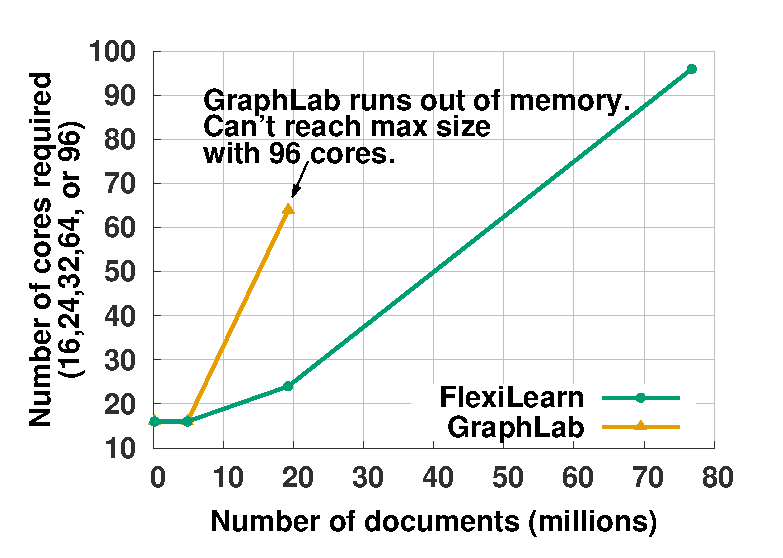
\includegraphics[width=0.46\textwidth]{fig2/lda_machines_failing.eps} 
\caption{The minimum number of machines needed vs the data size. We can see that \ourmethod 
is economic compared to graphlab for a given data size}
\label{fig:ldaMachinesNeeded}
\end{figure}



\begin{figure*}[t]
\centering
\begin{tabular}{|c|c|c|c|}
\hline
\multicolumn{4}{|c|}{\bf Topic Modeling} \\
\hline
Convergence Plots & \# of Topics & \# of Processors & \# of Docs \\
\hline
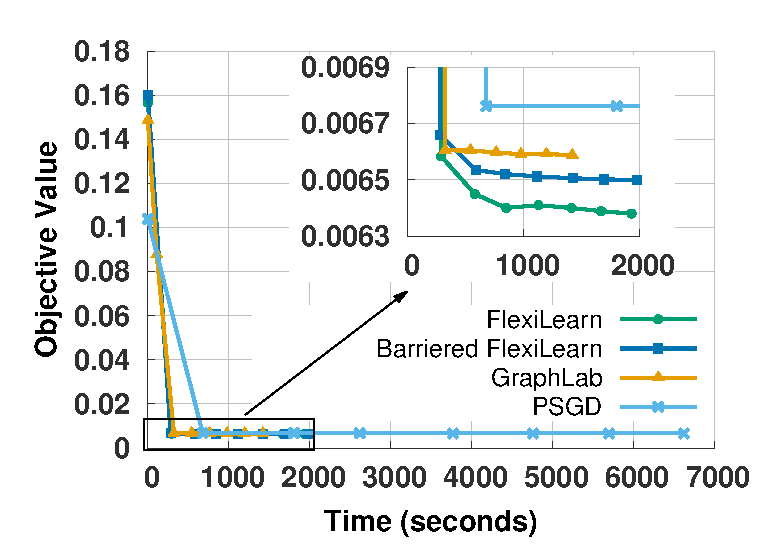
\includegraphics[width=0.23\textwidth]{fig2/lda_convergence.eps} &  
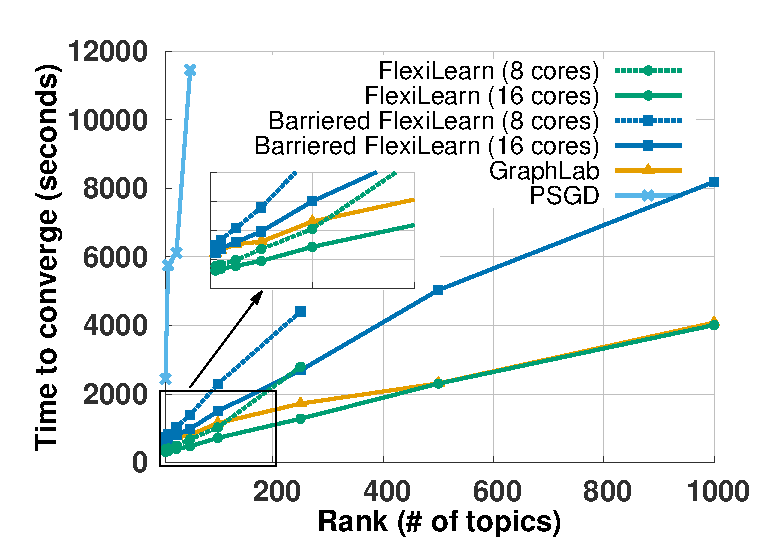
\includegraphics[width=0.23\textwidth]{fig2/lda_rankv3.eps} & 
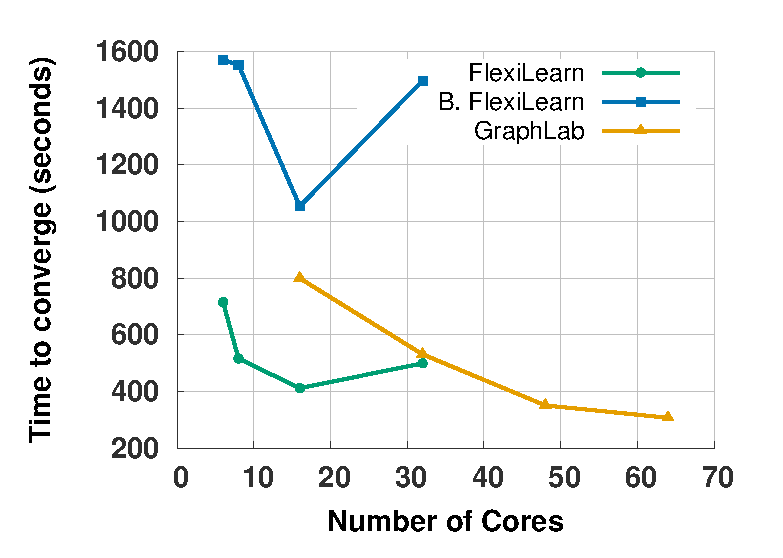
\includegraphics[width=0.23\textwidth]{fig2/lda_machines.eps} &
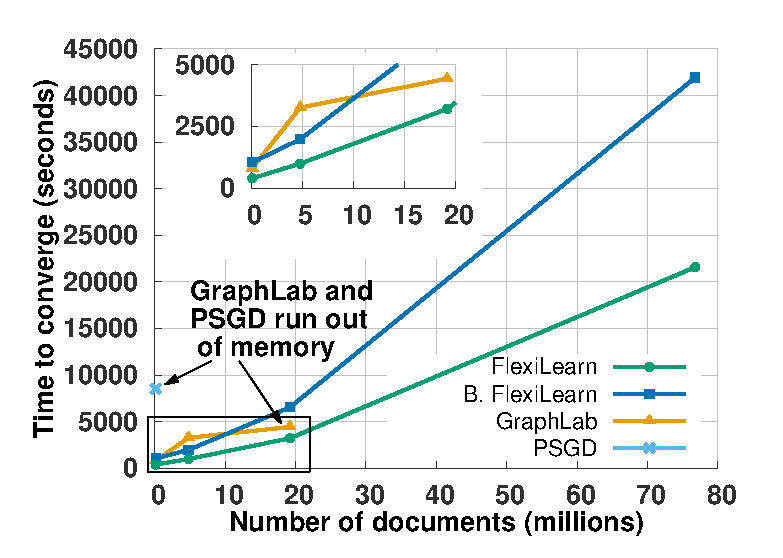
\includegraphics[width=0.23\textwidth]{fig2/lda_datasize.eps} \\
\hline
\multicolumn{4}{|c|}{\bf Dictionary Learning} \\
\hline
Convergence Plots & \# of Dictionary Bases & \# of Processors & \# of Images \\
\hline
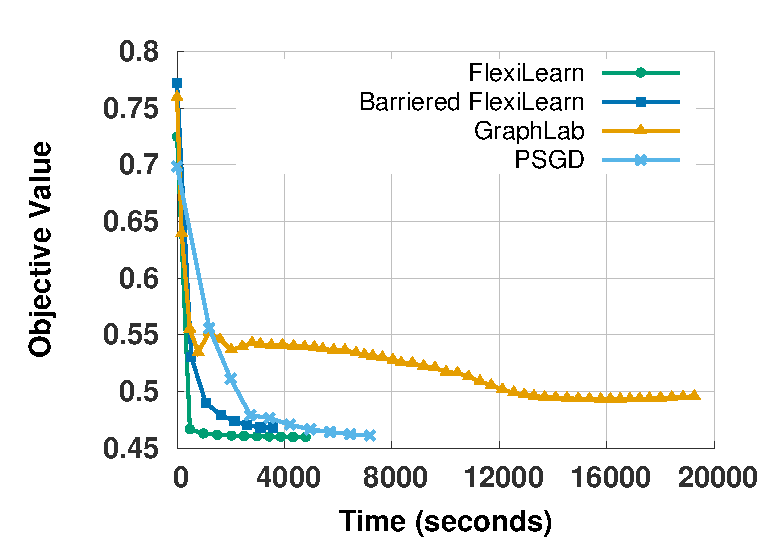
\includegraphics[width=0.23\textwidth]{fig2/dict_convergence.eps}& 
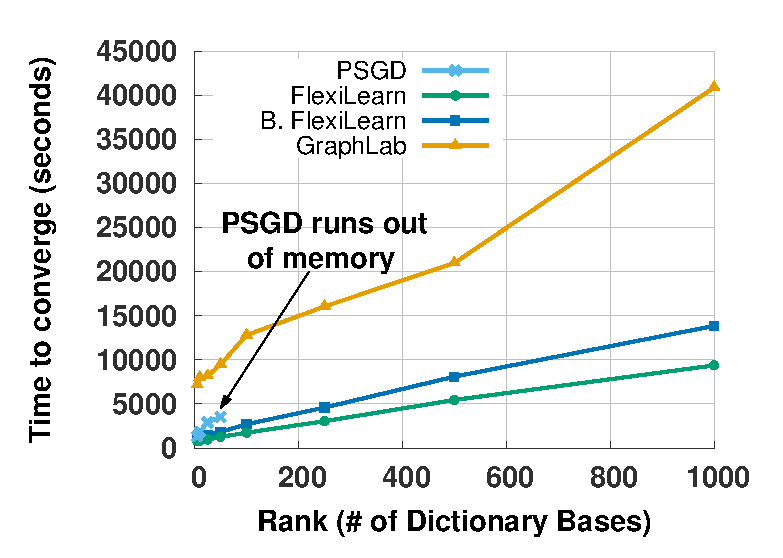
\includegraphics[width=0.23\textwidth]{fig2/dict_rank.eps} & 
TODO &
%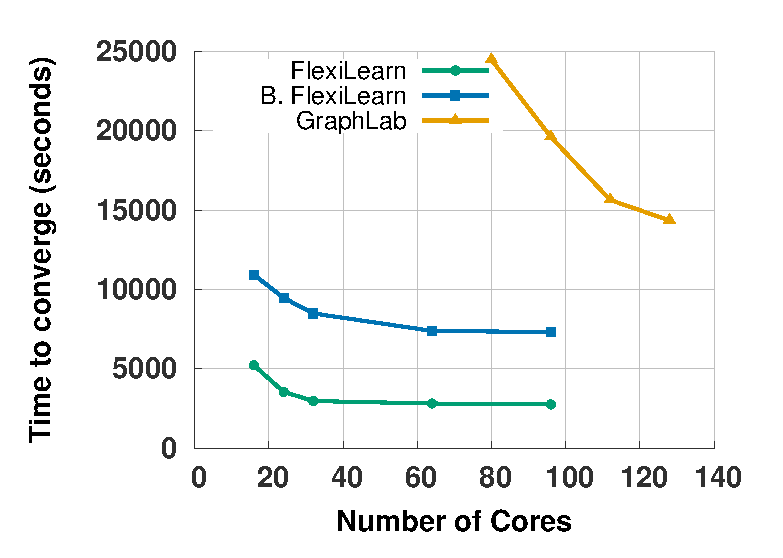
\includegraphics[width=0.23\textwidth]{fig2/dict_machines.eps} &
\includegraphics[width=0.23\textwidth]{fig2/dict_datasize.eps} \\
\hline
\multicolumn{4}{|c|}{\bf Mixed Membership Network Decomposition} \\
\hline
Convergence Plots & \# of Network Roles & \# of Processors & \# of Network Nodes \\
\hline
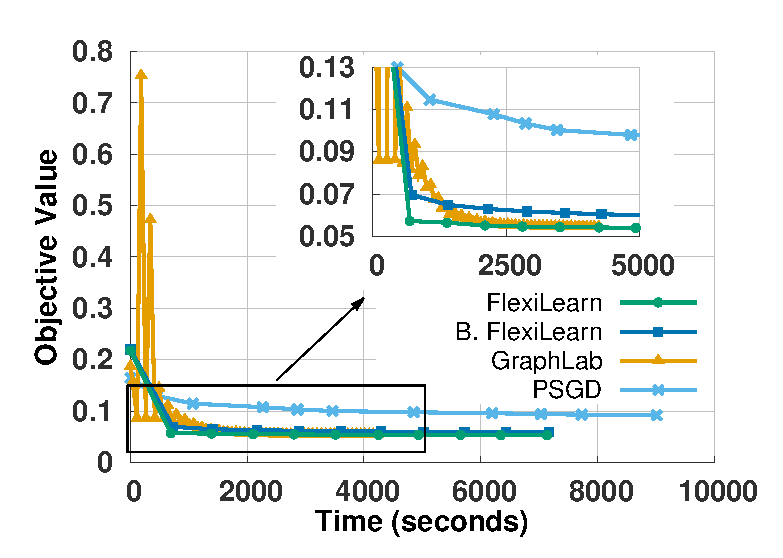
\includegraphics[width=0.23\textwidth]{fig2/mmsb_convergence.eps} &
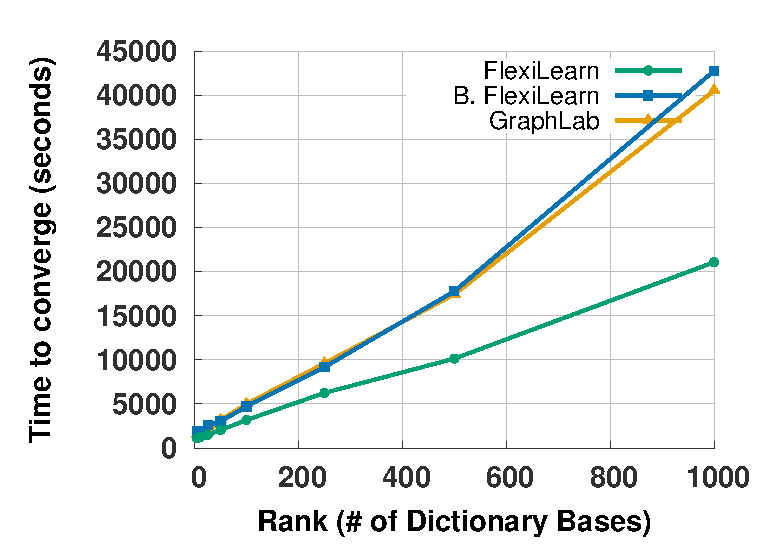
\includegraphics[width=0.23\textwidth]{fig2/mmsb_rank.eps} & 
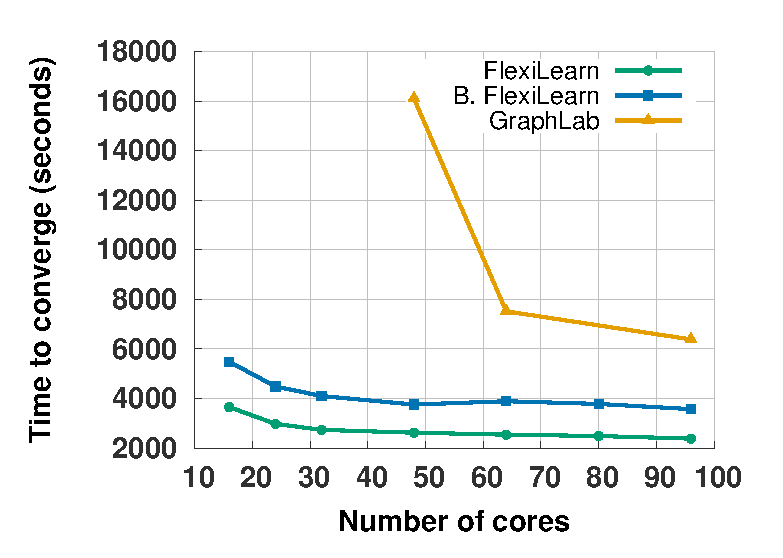
\includegraphics[width=0.23\textwidth]{fig2/mmsb_machines.eps} &
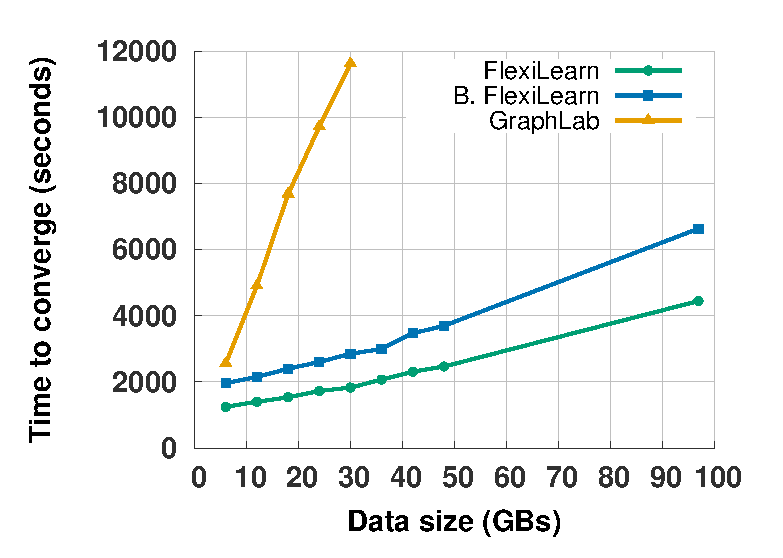
\includegraphics[width=0.23\textwidth]{fig2/mmsb_datasize.eps} \\
\hline
\end{tabular}
\caption{\small Convergence (Left) and scalability (in rank, processor cores and data size)
of all methods, on topic modeling, dictionary learning and mixed-membership network decomposition.
The convergence plot reveals the solution trajectory of each method, revealing pathological behavior such as oscillation.
The scalability plots show how each method fares as the problem rank, number of processor cores, and data
size is increased.}
\label{fig:results}
\end{figure*}

\subsection{Hardware Specifics} The Hadoop cluster used has 
2x Intel Xeon E5440@ 2.83GHz (8 cores per machine) machines each with 16GB RAM and 10Gbit
Ethernet. All three Hadoop based methods  (\ourmethod, \dsgd and \psgd) run on this cluster.
\graphlab is run on a different cluster as the Hadoop cluster didn't support MPI. The 
\graphlab cluster consists 2x Intel Xeon E5-2450 @2.1-2.9GHz (16 cores per machine)  with
128GB RAM and 10Gbit Ethernet. Thus \graphlab experimental setup has more memory but slightly 
slower machines.

%\abhi{note down which dimensions (dimensions, rank, machines, density) are fixed to what 
%for which experiments}


\section{Evaluation} % (fold)
\label{sec:eval}

\begin{figure}[t]
\vspace{-0.4cm}
\centering
\begin{tabular}{|c|c|}
\hline
 \multicolumn{2}{|c|} {\bf Time taken to converge} \\
\hline
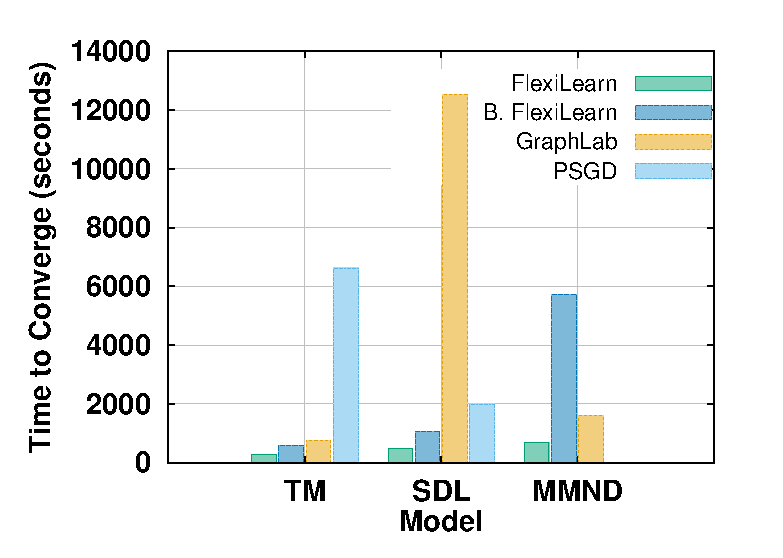
\includegraphics[width=0.46\columnwidth]{fig2/speedup.eps} &
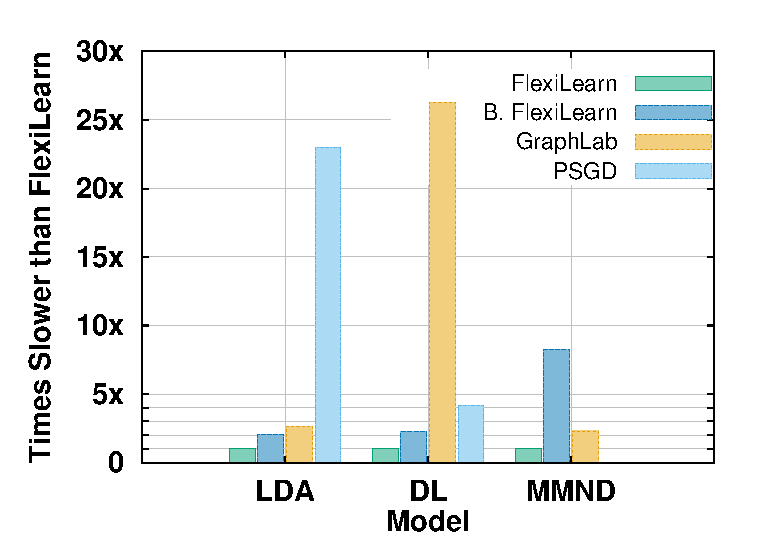
\includegraphics[width=0.46\columnwidth]{fig2/speedup2.eps} \\\hline
\end{tabular}
\vspace{-0.3cm}
\caption{\small Time taken by all methods to converge on the
three ML models, on an absolute scale (left) as well as a relative scale (right).
The methods plateau at these values in the respective plots shown
in Figure~\ref{fig:results}. The bar for \psgd is absent in the figure as it never reaches $0.059$ and stops around 
objective value $0.092$.  }
\label{fig:speed}
\end{figure}

\begin{figure}[t]
\vspace{-0.1cm}
\centering
\begin{tabular}{|c|c|}
\hline
 \multicolumn{2}{|c|} {\bf Break up of time take to finish tasks in reducer} \\
\hline
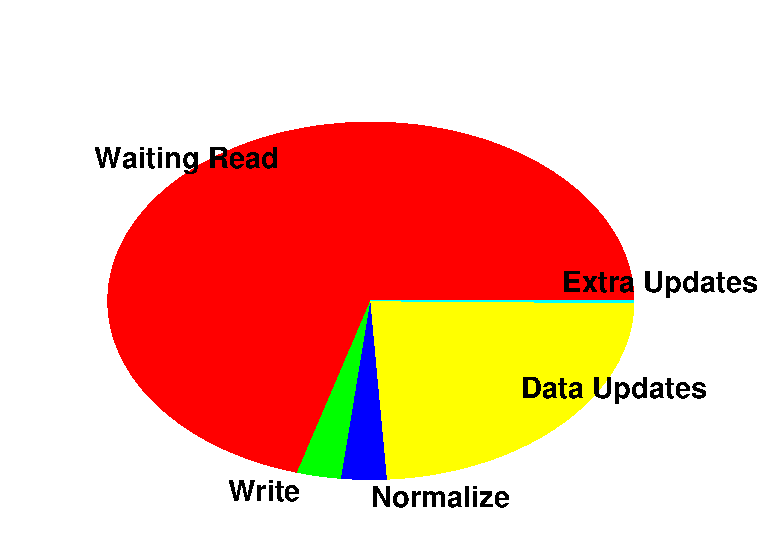
\includegraphics[width=0.46\columnwidth]{fig2/lda_piechart.eps} &
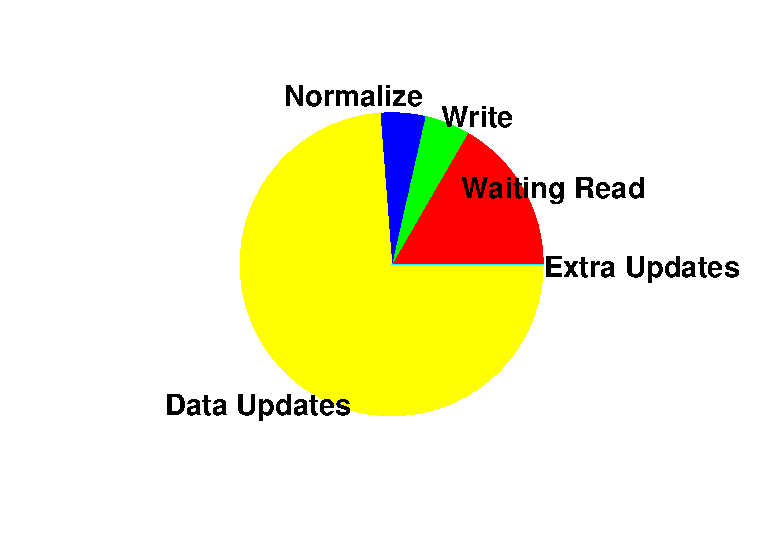
\includegraphics[width=0.46\columnwidth]{fig2/mmsb_piechart.eps} \\\hline
\end{tabular}
\vspace{-0.3cm}
\caption{\small Proportional breakup of time taken during different tasks in the 
reduce phase. The left hand graph is for \lda with 32 processors and \snytimes{32} 
dataset	and the right hand plot is for \mmsb with 32 processos and \swebgraph{8}
dataset. ``Waiting Read" is time a reducer waits to synchronize with other 
reducer to finishing 
writing its updates. ``Normalize" is the time taken to ensure the normalization constraints
for \lda and \mmsb, 
``Write" is the time taken to write the intermediate factors and output files to 
hdfs, ``Data Updates" is the time takes to perform computations on the 
data, and ``Extra Updates" is the time taken to perform extra updates while waiting 
for to synchronize with other reducers.
We can see that time for waiting to read is more than time for data updates 
in case of \lda due to distributed normalization. }
\label{fig:piechart}
\end{figure}

All four learning \schemes are evaluated on three criteria: 
1) their speed, 2) scalability (in data size as well as 
model size), and 3) quality of answers. We see that \ourmethod outperforms all 
other schemes with huge margins on all three \queries \abhi{we call the three models as 
queries} and over all three criteria.


\subsection{Scalability}
Columns two, three and four in Figure~\ref{fig:results} show the scalability of different
methods in model size, number of machines and data size for all three \queries. We see
that \ourmethod performs quite well across the spectrum. 

%\vspace{-0.4cm}
%\section{Experiments}
%\vspace{-0.3cm}
%
%\begin{figure*}[t]
%\vspace{-0.4cm}
%\centering
%\begin{tabular}{|c|c|c|c|}
%\hline
%\multicolumn{2}{|c|}{\bf Topic Modeling} & {\bf Dictionary Learning} & {\bf MMND} \\
%\hline
%Convergence Plots & Scaling in \# Cores & Convergence Plots &  Convergence Plots \\
%%\multicolumn{4}{|c|}{\bf Topic Modeling} \\
%%\hline
%%Convergence Plots & \# of Topics & \# of Processors & \# of Docs \\
%\hline
%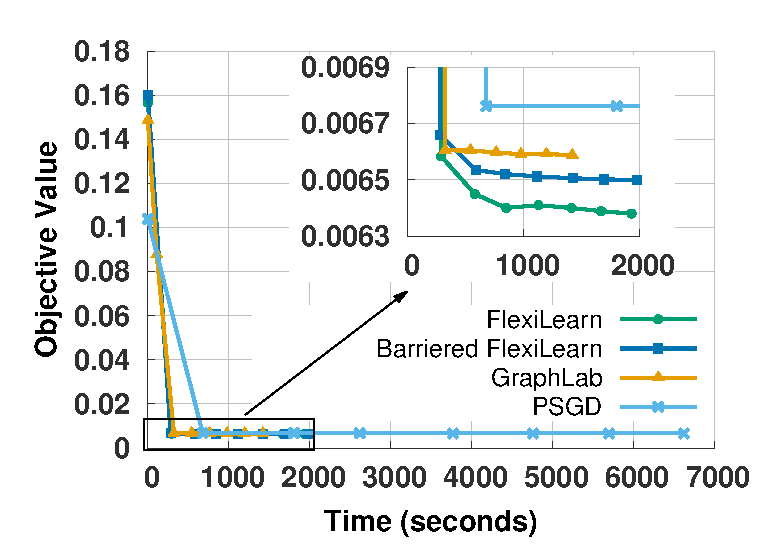
\includegraphics[width=0.23\textwidth]{fig2/lda_convergence.eps} 
%& 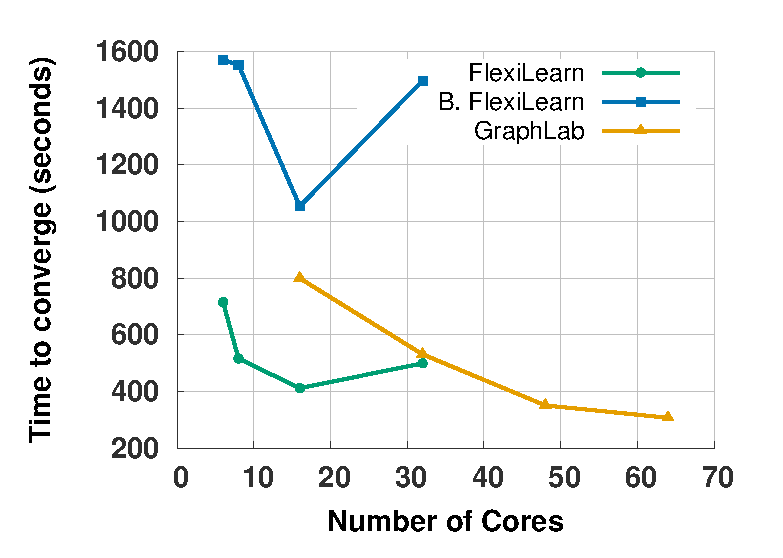
\includegraphics[width=0.23\textwidth]{fig2/lda_machines.eps} 
%& 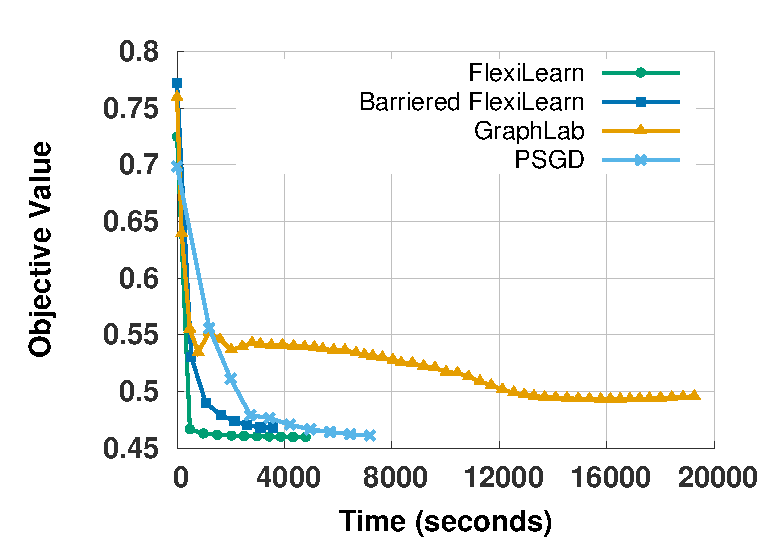
\includegraphics[width=0.23\textwidth]{fig2/dict_convergence.eps} 
%& 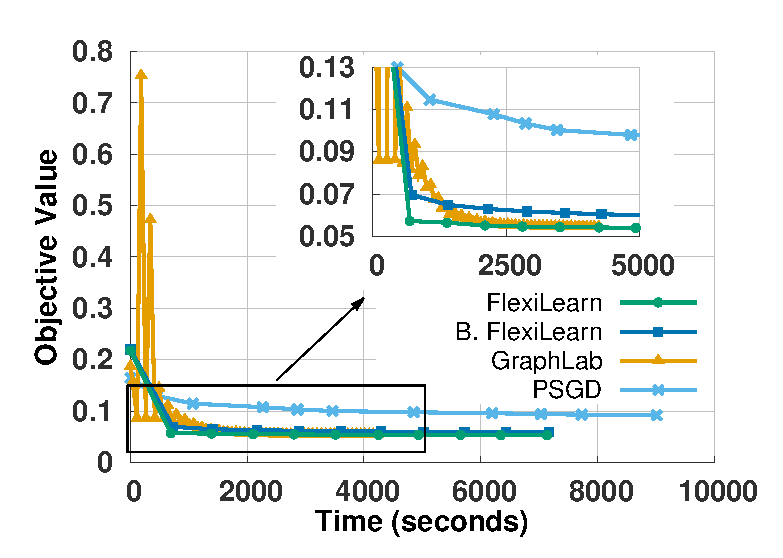
\includegraphics[width=0.23\textwidth]{fig2/mmsb_convergence.eps}  
%\\
%\hline
%%{\bf Topic Modeling} & {\bf Dictionary Learning} & \multicolumn{2}{|c|}{\bf Mixed Membership Network Decomposition} \\
%\multicolumn{4}{|c|}{\bf Topic Modeling} \\
%\hline
%Machines Needed & Scaling in \# Docs & \multicolumn{2}{|c|}{Scaling in \# Topics} \\
%\hline
%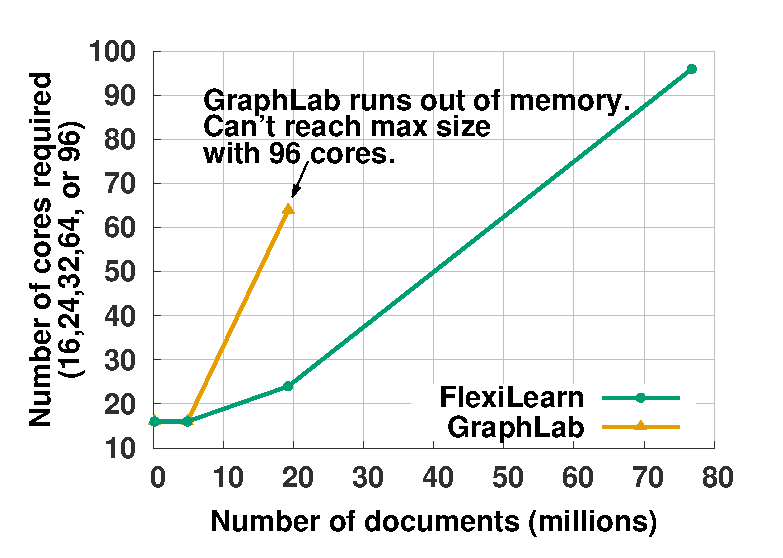
\includegraphics[width=0.23\textwidth]{fig2/lda_machines_failing.eps}
%& 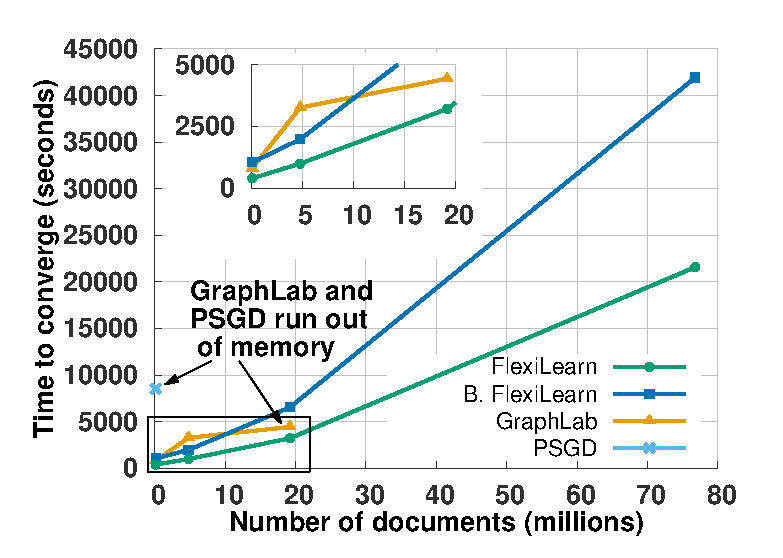
\includegraphics[width=0.23\textwidth]{fig2/lda_datasize.eps}
%& \multicolumn{2}{|c|}{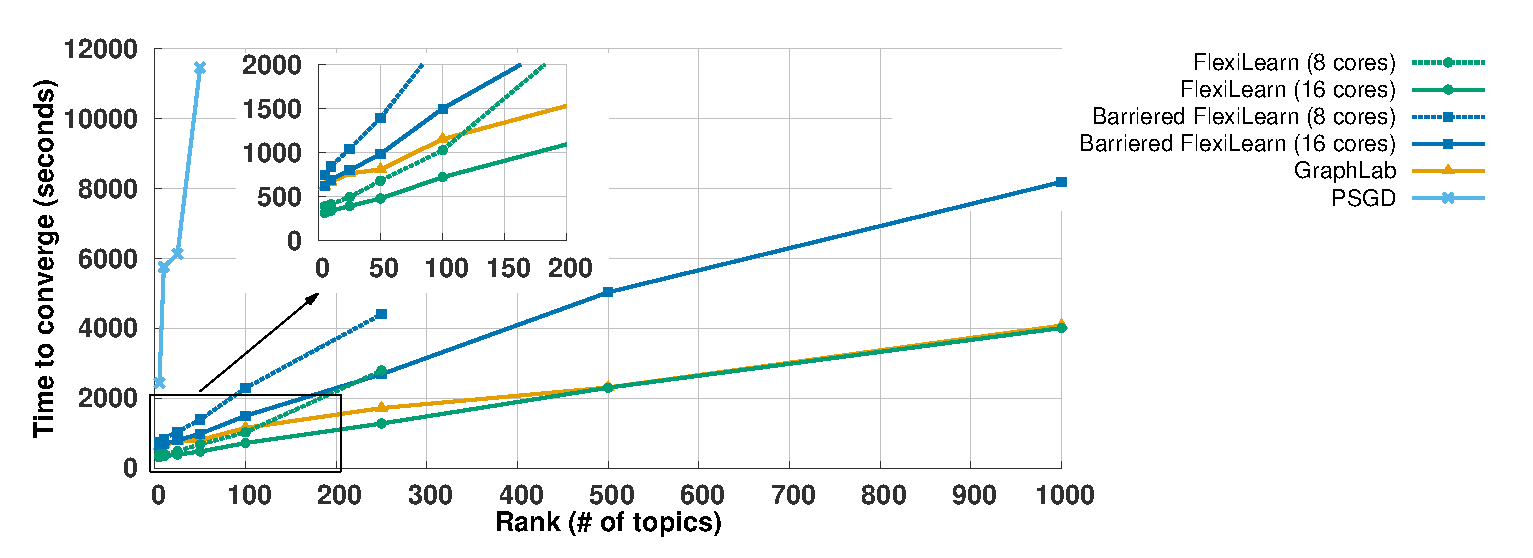
\includegraphics[width=0.46\textwidth]{fig2/lda_rankv2.eps}} \\
%\hline
%\end{tabular}
%\vspace{-0.3cm}
%\caption{\small Convergence and scalability plots for the three models (\lda, \dl, \mmsb),
%under our \ourmethod{} and baselines (\dsgd, \psgd, \graphlab). Unless otherwise stated in the plot, all methods were run with 16 cores
%and rank $K=25$. For all topic modeling plots except ``\# of Docs" and ``Machines Required", we used the NyTimes4 dataset (Table \ref{tab:dataset}).
%The convergence plots reveal the objective trajectory and final value of each method,
%while the scalability plots show how each method fares (on topic modeling) as we increase the problem rank, number of processor cores, and data size.
%In the bottom left, we also show the minimum number of machines required for a given topic modeling dataset size, for
%\ourmethod{} and \graphlab.}
%\vspace{-0.5cm}
%\label{fig:results}
%\end{figure*}

\paragraph{Dataset size}
For data size scalability experiment, we fix the number of processors as 32 
and rank as 25 for all three \allmethods and all three. 
Column four of Figure~\ref{fig:results} shows the convergence time taken by the different
\schemes with respect to increasing data size. We vary the data size in two ways: 1) by 
making the data denser e.g. increasing the number of edges in the graph (or 
entries in the adjacency matrix ) for  
\mmsb instead of increasing the number of vertices, 
and 2) by increasing the dimensions of the data e.g.
increasing the 
number of documents. In this set of experiments we vary the \lda and \sdl data 
size by increasing the number of documents. For \mmsb we increase the data by making it 
denser with inclusion of more edges as explained in section~\ref{subsec:data}. 
A subtle distinction between the two ways of increasing size is that increasing the dimension of 
the data also increases the model size e.g. for the document by word input count matrix 
for \lda, increasing the columns (number of words) increases the size of 
topic-word model parameter. 
This has bad repercussions for an approach
that is only scalable in data e.g. \psgd. 
\psgd runs out of memory very early (for data of size 6 GBs) 
in the data-size experiments for \lda and \sdl since the parameters also 
increase with the increase in size of the data. For \mmsb it keeps running 
with increase in size for a while although with poor convergence. 
It doesn't reach the convergence threhold and hence is
not included in the plots. Our \ourmethod scales well for both ways of increasing 
data size. It never runs out of memory in any of the \query types for sizes shown in the 
figure as well as is faster by at least a factor of 2. Figure~
\ref{fig:ldaMachinesNeeded} shows a comparison of number of machines needed for \ourmethod
and \graphlab for \lda. Figures~\ref{fig:results} and \ref{fig:ldaMachinesNeeded} 
combined show that not only 
\ourmethod is faster but also requires fewer processors for a given data size. 
Alhough like the other three \allmethods, it stores all its variables in 
memory for computation. This speed and economy stems from the fact that \ourmethod 
is distributed over both data and model, unlike \graphlab which is distributed over 
vertices that may not corresspond to data and model distribution. Or unlike 
\psgd that only is distributed over data and not model.  
%\alex{we need to be more concrete here and explain that we are all memory based
%systems}


\paragraph{Model parameters}
The model parameter are the types of variables that arise as a construct of the model (
Section~\ref{subsec:abstractProblem}). For example, the number of topics 
in \lda or the number of basis vectors in \sdl is a construct of the model.  
Column two shows the variations for different models for increase in rank (topic, bases or
network role number). For this set of experiments we fix number of processors as 16 for all 
\allmethods and \queries. 
The datasets used are \snytimes{4}, \swebgraph{1}, and \imagenet for \lda,
\mmsb and \sdl respectively.
Here again we see that \ourmethod is faster to converge than all the other
\allmethods. The difference in convergence rate of \graphlab and \ourmethod is especially stark
for \sdl. The reason for this is that \graphlab oscillates by huge margins for this problem as
seen in Figure~\ref{fig:results}, second row, first column. 
\psgd runs out of memory quite early (for rank 100) as expected for \lda and \sdl.
Since the dimensions of the \mmsb data are smaller (281,904) that \lda (1,200,000) or \sdl
(1,261,406), \psgd runs out of memory a little later (for rank 200) for this \mmsb \query. 

\paragraph{Processors}
Column three shows the effects of varying number of processors for a fixed data and model size.
We have set rank as 25 and used \snytimes{32}, \swebgraph{8}, and \simagenet{4}
as data sets for \lda, \mmsb, and \sdl. 
We scale well in terms of processors needed for larger data sets for \lda compared to \graphlab.
We observe that for smaller data sizes \ourmethod gradually starts giving 
diminishing returns with increasing processors in case of \lda and its curve
is worse than \graphlab. But for larger datasets \ourmethod
has the best curve. This happens due to the fact that for smaller dataset time taken to synchronize 
among the reducers dominates the time taken to perform computations on the data. 
This fact is also illustrated in figure~\ref{fig:piechart}. 
Figure~\ref{fig:piechart} shows a break up of the percentage of time each reducer
spends on different tasks. For \lda every reducer has to perform 
distributed projections defined in \ref{sub:Computation}. To achieve this a reducer has to poll 
all the other reducers at the end of every subepoch, leading to 
extra waits compared to a non-distributed projection.  
The effects of this wait is more pronounced for \dsgd as it performs much worse 
(figure~\ref{fig:results}, column three, row one). Our method due to its provably correct Always-On property
mitigates the ill effects of sync-waits by doing more work.
For \mmsb its 
time spent on computation is the highest among all its tasks. As there is far fewer 
synchronization to be done. Though there is still synchronization happening between two 
consecutive blocks in a sub-epoch where reducer in block $i$ is waiting for reducer in 
block $i+1$ to finish so that reducer in $i$ can move to block $i+1$ 
in the next sub-epoch.
The actual number of datapoints updated in the ``Extra Updates" are 950,760 (of $10.3*10^9$ 
total data points) and 14,556,089 (of $3.2*10^9$ total data points) per 
reducer (in total 32 reducers) per epoch. 
In case of \sdl and \mmsb, \ourmethod performs significantly well compared to others.
For these set of experiments \psgd doesn't converge to the optimal point as more 
machines are added due to its bad averaging guarantees
on non-convex problems~\cite{zinkevich2010parallelized}. It is significantly slower too
since all the variable after independently being computed in the 
update phase on $d$ reducers ($d=32$ here) are passed through a single 
reducers for averaging and thus
creating a bottleneck.  

\subsection{Convergence speed}
Figure~\ref{fig:speed} shows convergence times 
for \ourmethod{}, \dsgd, \psgd, and \graphlab over the three 
models: \lda, \mmsb and \dl. \ourmethod{} is faster
by anywhere between $2.6\times$ (vs \graphlab on \lda) 
to $26.2\times$ (vs \graphlab on \sdl). This clearly is due to the Always-On 
property of \ourmethod.
The number of reducers used is 16 and the datasets are \snytimes{4}, \swebgraph{1} and 
\imagenet. 
%\begin{figure}[t]
%\vspace{-0.4cm}
%\centering
%\begin{tabular}{|c|c|}
%\hline
% \multicolumn{2}{|c|} {\bf Time taken to converge} \\
%\hline
%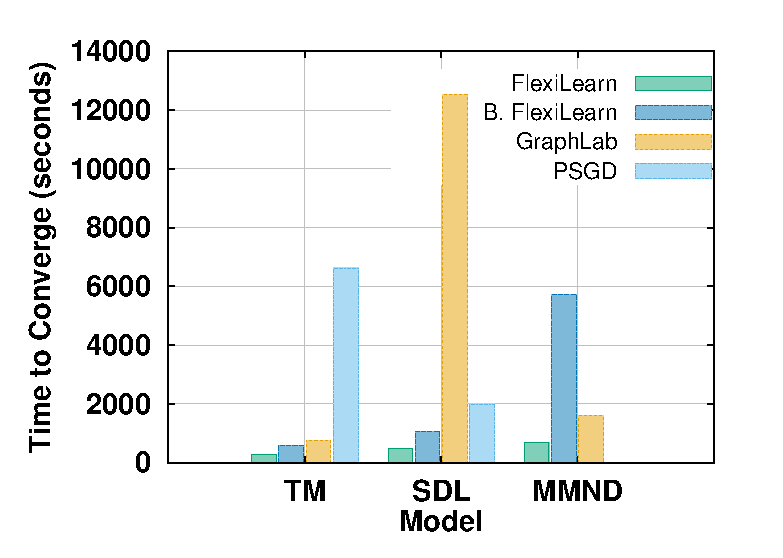
\includegraphics[width=0.46\columnwidth]{fig2/speedup.eps} &
%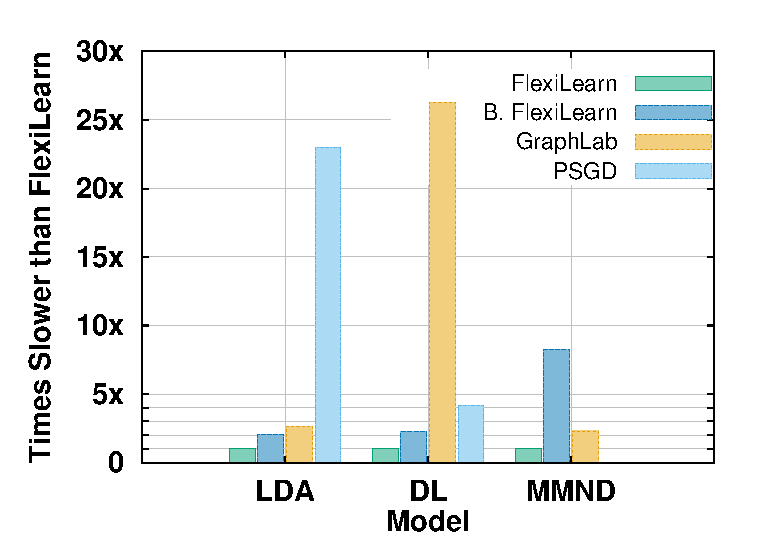
\includegraphics[width=0.46\columnwidth]{fig2/speedup2.eps} \\\hline
%\end{tabular}
%\vspace{-0.3cm}
%\caption{\small Time taken by all methods to converge on the
%three ML models, on an absolute scale (left) as well as a relative scale (right).
%The methods plateau at these values in the respective plots shown
%in figure~\ref{fig:results}. The bar for \psgd is absent in the figure as it never reaches $0.059$ and stops around 
%objective value $0.092$.  }
%\label{fig:speed}
%\end{figure}

\subsection{Convergence quality}
The number of processors used is 16 and rank is 25 for all three \allmethods and \queries.
The datasets used are \snytimes{4}, \swebgraph{1}, and \imagenet for \lda,
\mmsb and \sdl respectively.
Though graphlab is large scale and is a distributed work load system, it has no theoretical 
guarantees. This shows up in the quality of answers we get. \ourmethod is distributed, faster,
better scalable, and gives higher quality of answers. Figure~\ref{fig:results}, 
column one shows the convergence curve for all the approaches on all three problems.
\ourmethod achieves better convergence value with faster speed compared to others. 
The higher quality of results stems from the fact that \ourmethod is 
guaranteed to be correct theoretically. \graphlab oscillates quite a lot for \mmsb and \sdl. 
This is due to  the fact that it updates vertices in partitioned sets without any guarantees
for the constraints (as discussed in Section~\ref{sec:complexQues})
%\graphlab oscillation reasons and patterns, \dsgd and \psgd converges to a poor
%quality,
\subsection{Why \ourmethod outperforms other approaches}
\ourmethod wins emphatically on all three criteria, and on all three problems is due to 
following properties:
\begin{itemize}
\item Unlike \psgd, it is distributed over data as well as model. This gives \ourmethod 
atleast twice the speed as well as scalability compared to \psgd 
\item Unlike \graphlab, it is theoretically grounded. This gives \ourmethod a guarantee 
for high quality answers
\item Unlike \dsgd it does not waste time while waiting to synchronize. This makes it 
more scalable (as we saw in case of machine scalability) and faster by several factors of
magnitude.
\end{itemize}
%Put a plot of waiting times in different concstraints case and argue why it
%helps here.


\section{Related Work} % (fold)
\label{sec:related}
We started with the premise of solving big models over big data, 
but in the current state of the art there are very few works 
that handle both. The big data focus is mainly on i.i.d (identical
and independently distributed) 
nature of the datasets. This informally means that there is no probabilistic 
difference between any two randomly picked samples of the data.
\psgd ~\cite{zinkevich2010parallelized} exploits this property by 
partitioning the data randomly, computing variables on each partition 
independently, and finally averaging them in the end. 
This has an advantage that there is no communication 
needed between the machines until the final phase when they all have converged 
and are ready to synchronize.
But this does not work well when the problem size
is bigger (e.g. when we increase the number of topics 
in \lda). The other class of algorithms in this category are 
fixed-delay algorithms~\cite{agarwal2012distributed,langford2009slow}. 
Here, there is a central server that facilitates communication between machines 
in a fixed ordering. But this suffers with the slow worker bottleneck problem
where slower machines or failed machines dictate the system speed.

In most ML problems each variable is dependent on 
a small set of other variables. When faced with a big model 
the general approach in the current literature is to exploit 
this proeprty. This is the philosophy behind \graphlab
~\cite{low2012distributed} as well as Google Brain project
~\cite{dean2012large}. \graphlab defines every variable as a vertex 
in a graph and partitions them into sets for distributed processing.
But as we have shown, the speed up gained in this case is sub-optimal 
since these partitions may not correspond to an efficient partition
along data and model dimensions. In case of Google Brain project 
the corresponding paper does not detail any generic partitioning 
strategy. Moreover none of the above are
theoretically well grounded. Though Hogwild paper~\cite{niu2011hogwild} provides
theoretical analysis of parallel updates of the same variable in two different 
processors, it does not provide a generic partitioning strategy or any analysis 
in that direction. Besides their experiments only cover single machine
with multiple cores. 


In the present ML systems literature there are no existing works that achieve 
scaling in data as well as model for general ML probelms.
Even for specific problems there are very few cases such as distributed matrix factroization 
by Gemulla et al.~\cite{Gemulla:2011:LMF:2020408.2020426}. 
This is the work that is closest to \ourmethod, but they are restricted to
matrix factorization.
We also differ from this work in providing a 
a generic partitioning strategy for arbitrary machine learning problems and 
allowing workers to run over barriers to avoid the negative impact of stragglers. 

Another useful class of ML systems are parameter servers that are based on distributed
shared-memory interface and is helpful for large number of model parameters
~\cite{ahmed2012scalable,power2010piccolo}. However they lack a generic variable scheduling 
strategy. Recent works on parameter servers have come up with stale synchronous parallel (SSP) 
schemes~\cite{ho2013more,cipar2013solving} that reduce inter-machine communication
mitigating the effects of slow workers. The difference between SSP and \ourmethod is that 
SSP reduces communication regardless of the scheduling strategy, where as \ourmethod intelligently 
partitions and schedules variable updates to mitigate slow workers. 
\ourmethod can be used in conjuntion with SSP to provide further improved answers to 
bigger data and model questions. 

%\ourmethod does not scale well in number of machines if the data 
%size is small. In such a scenario the synchonization time dominates every 
%thing else (Figure~\ref{fig:piechart}). This stems from the 
%limitation of using Hadoop. A system that can ensure few inter-machine 
%communications (e.g. SSP) can help \ourmethod overcome this. We plan to 
%explore this as future work.  
%Another problem is: in case of pathalogically skewed load distribution 
%between the machines or in case a mahine dies altogether, the guarantess 
%of \ourmethod may not hold. These can be solved by sorting the data for 
%fair load scheduling prior to 
%running \ourmethod. 

\ourmethod provides a generic partitioning and schedulng strategy
that is distributed on data as well as model size. Its firm theoretical
standing ensures better annswers whereas its ability to distribute both the
data and model guarantees faster answers. These attributes have been justified
We have demonstrated empirically that \ourmethod successfully converges faster
and to better results than state of the art competitors on multiple complex
machine learning applications.
%emprically (Section ~\ref{sec:eval}).
%But there are certain areas that need further improvement such as machine 
%scalability over smaller datasets and load balancing. 


\section{Conclusion} % (fold)
\label{sec:conclusion}
\ourmethod provides a generic partitioning and schedulng strategy
that is distributed on data as well as model size. Its firm theoretical
standing ensures better annswers. 
And its distributivity over data and model guarantees
faster answers. These attributes have been justified emprically ( 
section ~\ref{sec:eval}) as well as theoretically~\cite{theoryResult}.
Though there are certain areas that need further  
improvement. 

\ourmethod does not scale well in number of machines if the data 
size is small. In such a scenario the synchonization time dominates every 
thing else (figure~\ref{fig:piechart}). This stems from the 
limitation of using hadoop . A system that can ensure few inter-machine 
communications (e.g. SSP) can help \ourmethod overcome this. We plan to 
explore this as future work.  Another problem is: in case of pathalogically skewed load distribution 
between the machines or in case a mahine dies altogether, the guarantess 
of \ourmethod may not hold. These can be solved by sorting the data for 
fair load scheduling prior to 
running \ourmethod. 


%{
%\small
\bibliographystyle{abbrv}
\bibliography{biblio}
%}


\end{document}
